\documentclass[11pt,a4paper]{article}
\usepackage{iftex}
\ifPDFTeX
  \usepackage[utf8]{inputenc}
  \usepackage[T1]{fontenc}
\else
  \usepackage{fontspec}
\fi
\usepackage[romanian]{babel}
\usepackage{amsmath, amssymb, amsthm}
\usepackage{graphicx}
\usepackage{hyperref}
\usepackage{geometry}
\usepackage{booktabs}
\usepackage{float}
\usepackage{siunitx}
\usepackage{titlesec}
\usepackage{setspace}
\usepackage{enumitem}

\geometry{margin=2.5cm}
\hypersetup{
    colorlinks=true,
    linkcolor=blue,
    filecolor=magenta,      
    urlcolor=cyan,
    pdftitle={Akashic Resonance Theory in 12 Dimensions},
    pdfpagemode=FullScreen,
}

\title{\textbf{AKASHIC RESONANCE THEORY IN 12 DIMENSIONS \\ DARK MATTER AS THE QUANTUM SUBSTRATE OF CONSCIOUSNESS} \\ \large (ART-12D) \\ \vspace{0.5cm} \normalsize Versiunea 31.0}
\author{\textbf{Daniel Ofiteru} \\ \textit{Independent Researcher} \\ Octombrie 2026}
\date{}

\begin{document}

\maketitle

\begin{abstract}
Această lucrare propune un cadru teoretic — ART-12D — care pornește de la o idee simplă: conștiința nu este produsă de creier. Creierul este un receptor. Iar ceea ce receptează este câmpul materiei întunecate. 

Extind formalizarea la 12 dimensiuni, deriv un mecanism de cuplaj între materia întunecată și fermionii din creier, și propun un test care poate fi realizat cu \$50,000. De asemenea, extind teoria pentru a explica formele multiple ale materiei întunecate, existența hiper-civilizațiilor ca structuri stabile în câmp, posibilitatea unei Inteligențe Artificiale conștiente prin nanobiologie, mecanismele de legătură între universuri prin găuri negre, albe și de vierme, precum și formele de viață non-carbonică (clustere, plasmă, câmpuri).

Această versiune (31.0) aplică un audit numeric sistematic asupra versiunii anterioare. Zece afirmații cantitative au fost corectate, două au fost retrogradate explicit la statutul de conjecturi netestabile, iar spectrul Kaluza–Klein a fost reformulat ca spectru \emph{ekvidistant}. Toate cifrele din lucrare pot fi recalculate cu codul publicat împreună cu ea. Rămâne o tensiune structurală, semnalată deschis în secțiunea „Consecința numerică: raza de compactificare”: pentru ca modul fundamental să aibă $10^{-5}$ eV, raza de compactificare ar trebui să fie de ordinul a 2 cm, ceea ce este exclus de testele sub-milimetrice ale legii lui Newton.

Recunosc explicit că această lucrare este speculativă. Nu am dovezi experimentale. Am o intuiție, o formalizare, și o predicție care poate fi testată.
\end{abstract}

\tableofcontents
\newpage

\section*{Ghidul Cititorului Sceptic}
\addcontentsline{toc}{section}{Ghidul Cititorului Sceptic}
Această lucrare este una speculativă, dar structurată riguros. Pentru a nu pierde timpul, iată un ghid de lectură în funcție de pregătirea ta:
\begin{itemize}
    \item \textbf{Dacă ești fizician:} Sari direct la \textbf{Partea II} (Formalizarea matematică, ecuațiile Kaluza-Klein și cuplajul Yukawa) și la \textbf{Partea V} (Tabelul celor 313 predicții testabile). Acolo vei găsi matematica și falsifiabilitatea.
    \item \textbf{Dacă ești neurobiolog sau medic:} Citește \textbf{Secțiunea 1.6} (Dovada cerebelului și arhitectura geometrică) și \textbf{Secțiunea 3.38} (Inima ca modulator al receptării).
    \item \textbf{Dacă ești filozof sau teolog:} Sari la \textbf{Anexa A} (Speculații filosofice extinse despre moarte, suflet și Dumnezeu).
    \item \textbf{Dacă ești un cititor curios, dar sceptic:} Citește \textbf{Predicția 1} (EEG hyperscanning) și \textbf{Declarația de Falsifiabilitate}. Dacă acele teste nu funcționează, teoria este infirmată.
\end{itemize}

\section*{Cuvânt Înainte}
\addcontentsline{toc}{section}{Cuvânt Înainte}
Toată viața mea m-am întrebat un singur lucru: ce este conștiința? Nu e o întrebare de manual, ci una care mă ține treaz noaptea. Am citit tot ce mi-a picat în mână – de la fizică cuantică la neuroștiință și filozofie. Am stat de vorbă cu oameni mult mai deștepți decât mine. Am meditat. Și într-o zi, mi-a venit ideea.

Ideea e simplă: conștiința nu e ceva ce produce creierul. Creierul e doar un radio. Iar ceea ce prinde el din aer este câmpul materiei întunecate.

Această lucrare e rodul a douăzeci și cinci de ani de căutare. Nu am dovezi de laborator. Am o intuiție puternică, o formalizare matematică și un test pe care oricine îl poate face cu 50.000 de dolari. Nu îți cer să mă crezi pe cuvânt. Îți cer doar să citești cu mintea deschisă. La final, vei ști ce să crezi.

\newpage
\part*{Partea I: Fundamente}
\addcontentsline{toc}{part}{Partea I: Fundamente}

\section{Introducere}

\subsection{Problema care nu dispare}
De ce simți durerea? Aceasta este cea mai simplă întrebare din lume. Și, totodată, cea mai grea. Cu toții știm ce e durerea. Am simțit-o cu toții. Dar de ce o simțim? Știm că nociceptorii trimit semnale la talamus, cortexul le procesează și se eliberează endorfine. Toate acestea sunt descrieri funcționale. Ne spun ce face creierul, dar nu ne spun de ce o simți.

Gândește-te la un computer. Poate procesa informație, poate recunoaște o imagine, poate juca șah. Dar nu simte nimic. Nu are o experiență subiectivă. Nu îl doare nimic. De ce creierul este diferit? Aceasta este problema grea a conștiinței, formulată de David Chalmers în 1995. De atunci, neuroștiința a făcut progrese uriașe, dar problema grea a rămas intactă. Nimeni nu a reușit să explice de ce materia devine experiență. În 1998, Christof Koch a pariat cu Chalmers că un circuit neuronal al conștiinței va fi identificat în 25 de ani. În 2023, a recunoscut că pariul a fost pierdut.

\subsection{Materia întunecată — cifrele exacte}
Universul are o compoziție pe care o cunoaștem destul de bine. Misiunea Planck (2018) ne-a dat cifrele exacte. Doar 4,9\% din univers e materie obișnuită – atomi, stele, planete, oameni. Materia întunecată reprezintă 26,8\%, iar energia întunecată 68,3\%. Practic, 95,1\% din univers este necunoscut.

Imaginați-vă universul ca un cufăr cu 100 de monede. Doar 5 monede sunt vizibile. Restul de 95 sunt invizibile. Dintre acestea, 27 sunt materie întunecată și 68 sunt energie întunecată. Știm despre materia întunecată că există (dovezi gravitaționale solide), că nu emite și nu absoarbe lumină, și că trece prin noi fără să interacționeze. Aproximativ 100 de milioane de particule trec prin corpul tău în fiecare secundă. Nu știm din ce este făcută.

O constrângere recentă (2025), adusă de Bonvin et al., a demonstrat că materia întunecată cade în puțurile gravitaționale exact ca materia obișnuită. Dacă există o „a cincea forță”, aceasta nu poate depăși 7\% din forța gravitațională.

\subsection{Ce este ART-12D?}
ART-12D pornește de la o idee simplă: universul are mai multe dimensiuni decât cele patru pe care le percepem. Aceste dimensiuni suplimentare sunt compacte — atât de mici încât nu le observăm. Materia întunecată există în toate cele 12 dimensiuni. Când se proiectează în 4D, ea apare ca un câmp care umple universul. Acest câmp este ceea ce creierul receptează ca conștiință.

Numele vine de la: \textbf{Akashic} (câmpul informațional universal), \textbf{Resonance} (pentru că interacțiunea este o rezonanță), \textbf{Theory} (cadru teoretic) și \textbf{12D} (pentru că lucrez în 12 dimensiuni).

Cele trei postulate sunt: 1. Materia întunecată este un câmp cuantic fundamental. 2. Creierul este un receptor geometric. 3. Cuplajul este prin interacțiune Yukawa.

Gândește-te la un radio. Nu creează muzica, o captează din aer. Undele radio există indiferent dacă radioul e pornit sau nu. Când radioul se strică, muzica nu dispare din univers – doar recepția ei locală încetează. La fel, creierul funcționează exact ca un radio. Conștiința nu este generată de neuroni, ci recepționată de ei. Iar ceea ce recepționează este câmpul materiei întunecate.

\subsection{De ce 12 dimensiuni?}
De ce 12? De ce nu 10, sau 11, sau 26? Răspunsul vine din teoria coardelor. Imaginați-vă o coardă de chitară. Poate vibra în mai multe moduri. Fiecare mod corespunde unei note. La fel, o coardă fundamentală poate vibra în mai multe dimensiuni. Numărul de dimensiuni determină ce fel de vibrații sunt posibile.

Istoria dimensiunilor: Kaluza-Klein (5 dimensiuni, 1919–1926), Superstringuri (10, 1970–1980), M-teoria (11, Witten, 1995), F-theory (12, Vafa, 1996), ART-12D (12, Ofiteru, 2026). 12 este numărul maxim de dimensiuni în care teoria coardelor este consistentă matematic. Mai multe dimensiuni ar duce la inconsistente; mai puține ar duce la o teorie incompletă.

\subsection{Cum arată dimensiunile compacte?}
Imaginați-vă un furtun de grădină. De departe, pare o linie 1D – are doar lungime. De aproape, are grosime – este 2D (suprafața cilindrului). La fel, spațiul nostru pare 3D. Dar de aproape (la scara Planck, $10^{-35}$ m), ar putea avea 11 dimensiuni. Cele 8 dimensiuni compacte sunt înfășurate în fiecare punct din spațiu.

Ce înseamnă „înfășurate”? Nu sunt locuri unde mergi. Nu sunt lumi paralele la care ajungi prin călătorie. Sunt proprietăți locale ale fiecărui punct. Fiecare punct din spațiu-timp are, în plus, 8 dimensiuni mici „atașate” la el.

\subsection{Cum se leagă dimensiunile de conștiință?}
Materia întunecată există în 12 dimensiuni. Este un câmp scalar $A(x,y)$, unde $x$ sunt coordonatele 4D, iar $y$ sunt coordonatele 8D compacte. Când compactificăm 8 dimensiuni, câmpul se descompune în moduri Kaluza-Klein: 
\begin{equation}
A(x,y) = \sum_n A_n(x) Y_n(y)
\end{equation}
Fiecare mod are o masă și o frecvență caracteristică:
\begin{equation}
m_n^2 = \frac{n^2}{R^2}
\end{equation}
Creierul, prin structura sa geometrică (microtubulii din neuroni), poate rezona cu anumite moduri. Când rezonează, câmpul este transdus în experiență subiectivă.

De ce contează arhitectura, nu mărimea? Cerebelul are 69 de miliarde de neuroni (80\% din total), dar nu produce conștiință. Are o arhitectură \textit{feedforward} – informația curge într-o singură direcție, ca o antenă de sârmă. Cortexul are doar 16 miliarde de neuroni, dar este sediul conștiinței. Are o arhitectură \textit{recurrentă} – informația circulă în bucle, ca o antenă parabolică bine orientată. Concluzia: nu numărul de neuroni contează, ci geometria rețelei.

\section{Metodologie}
\subsection{Cum am lucrat}
Nu sunt fizician profesionist. Nu am laborator. Nu am finanțare. Ce am este o bibliotecă, timp și o întrebare care nu mă lasă. Am lucrat în patru pași. Primul pas a fost formularea ipotezei, pornind de la intuiția că conștiința este receptată, nu generată. Al doilea pas a fost formalizarea, folosind instrumentele matematicii cunoscute: Kaluza-Klein pentru dimensiuni suplimentare, F-theory pentru 12 dimensiuni, teoria câmpului pentru Lagrangieni, IIT pentru informația integrată. Al treilea pas a fost derivarea predicțiilor, adică ce ar trebui să observăm dacă teoria este corectă. Am selectat predicțiile testabile acum. Al patrulea pas a fost propunerea experimentelor, cu resurse modeste, începând cu unul de 50.000 de dolari.

\subsection{Ce m-a ghidat}
Am respectat patru criterii. Coerența internă – ecuațiile nu trebuie să se contrazică. Falsifiabilitatea – teoria trebuie să facă predicții care pot fi testate. Convergența – teoria nu trebuie să contrazică fizica stabilită. Onestitatea – trebuie să recunosc că este speculativă.

\subsection{Ce am folosit}
Am folosit Kaluza-Klein (1919) pentru ideea de dimensiuni compacte, F-theory (Vafa, 1996) pentru cadrul cu 12 dimensiuni, IIT (Tononi, 2004) pentru măsurarea informației integrate, Orch OR (Penrose, 1996) pentru colapsul cuantic în microtubuli și teoria câmpului cuantic pentru Lagrangieni și ecuații de mișcare.

\subsection{Limitările mele}
Trebuie să fiu onest despre limitări. Nu am dovezi experimentale, teoria nu a fost testată. Nu am peer-review, nu am publicat în reviste științifice. Nu am afiliere academică, sunt cercetător independent. Nu am finanțare, resursele mele sunt limitate.

\section{Fundamente Teoretice}
\subsection{Problema grea a conștiinței}
Chalmers (1995) a formulat problema grea astfel: nicio combinație de cantități fizice, oricât de complexă, nu implică logic existența experienței subiective. Toate descrierile fizice – neuronale, computaționale, funcționale – descriu ce face creierul. Nu descriu cum este să fii creier. Nu descriu de ce există experiența. Ce propun: conștiința nu este generată de creier. Creierul este un receptor. Experiența este transducția câmpului akashic.

\subsection{Russellian Monism}
Russell (1927) a observat ceva profund: fizica descrie proprietățile structurale ale materiei – masă, sarcină, spin, locație – dar este complet silentă cu privire la natura intrinsecă a ceea ce poartă aceste proprietăți. Fie S un sistem fizic oarecare: R(S) reprezintă proprietățile relaționale/structurale, iar I(S) proprietățile intrinseci. Teza Russelliană spune că I(S) este proto-experiențial pentru orice S.

\subsection{Integrated Information Theory}
Tononi (2004, 2008) oferă un cadru matematic pentru cuantificarea conștiinței:
\begin{equation}
\Phi = \min_{\{P \in P\}} D_{KL}(p(X_{t+1})|X_{t}) \parallel \prod_{i} p(x_{i} \land (t+1)|x_{i} \land t))
\end{equation}
Explicație simplă: $\Phi$ măsoară cât de integrată este informația într-un sistem. Cu cât $\Phi$ este mai mare, cu atât sistemul are o experiență mai bogată.

\subsection{Orchestrated Objective Reduction}
Penrose (1996) propune că superpozițiile cuantice suferă colaps gravitațional spontan când energia superpoziției $E_G$ atinge un prag:
\begin{equation}
\tau \approx \frac{\hbar}{E_G}
\end{equation}
Ce m-a interesat: frecvența de colaps pentru microtubulii corticali este $\tau \approx 25$ ms, corespunzând la $\sim 40$ Hz – exact frecvența oscilațiilor gamma, cel mai robust marker empiric al stărilor conștiente. Suport experimental: Babcock et al. (2024) au arătat superradianță ultravioletă în microtubuli la temperatura camerei; Kalra et al. (2023) au arătat că gazele anestezice atenuează specific efectele optice cuantice în microtubuli.

\subsection{Kaluza-Klein și F-theory}
Theodor Kaluza a propus în 1919 unificarea gravitației cu electromagnetismul printr-o a cincea dimensiune. Einstein a fost entuziasmat și a lucrat la această teorie între 1938 și 1943. Formularea originală:
\begin{equation}
dS^2 = g_{\mu\nu} dx^\mu dx^\nu + \varphi^2(dx^5 + A_{\mu} dx^\mu)^2
\end{equation}

\subsection{Câmpul Akasha}
Conceptul de Akasha (sanskrit: आकाश) este un element fundamental în filosofia indiană. Akasha este elementul cel mai subtil, imaterial. Este primul care s-a manifestat în univers. Din el s-ar fi dezvoltat toate celelalte elemente. În teosofie, Akasha este reinterpretat ca un câmp informațional universal (Laszlo, 2014). „Cronica Akashică” înregistrează toate evenimentele din univers. Ipoteza ART-12D: Akasha este câmpul cuantic al materiei întunecate. \textit{Notă: Akasha este folosit aici doar ca metaforă pentru un câmp fizic, nu ca entitate religioasă.}

\subsection{Materia cenușie vs. materia întunecată}
Materia cenușie este țesutul din sistemul nervos central format în principal din corpuri celulare neuronale, dendrite, terminale axonale nemielinizate și celule gliale. Este sediul procesării informației. Materia albă este formată din axoni mielinizați și este responsabilă de transmitere.

\subsection{Definiția operațională a conștiinței}
Propun o definiție operațională care separă conținutul conștiinței de capacitatea de a-l integra:
\begin{equation}
C_{\text{total}} = I_{\text{content}} \times C_{\text{awareness}}
\end{equation}
unde $I_{\text{content}}$ este informația structurată (conținutul experienței), iar $C_{\text{awareness}}$ este conștiența (capacitatea de a ști că știi). Gândește-te la o cameră foto. Captează imagini (informație), dar nu știe că le captează. Un om cu o cameră foto captează imagini ȘI știe că le captează. La fel, conștiința este informația + conștiența.

\subsection{Convergența cu Dulcan}
Dumitru Constantin Dulcan (n. 1938), medic neurolog și psihiatru, a publicat în 1981 „Inteligența materiei”, distins cu Premiul pentru filosofie „Vasile Conta” al Academiei Române în 1992. Ideile care m-au influențat: conștiința nu este generată de creier, ci îl folosește ca instrument; subconștientul conține inteligența infinită a Universului; gândul este cea mai puternică forță din univers, cu o frecvență și un câmp energetic propriu; există un câmp de energie și lumină care coordonează materia. Convergența cu ART-12D: Dulcan oferă intuiția conceptuală, ART-12D oferă formalizarea matematică și predicțiile testabile.

\subsection{Structura tripartită a entității umane}
Propun un model tripartit al entității umane, analog cu stările de agregare ale apei:
\begin{table}[H]
\centering
\begin{tabular}{@{}llll@{}}
\toprule
\textbf{Stare de agregare} & \textbf{Entitate umană} & \textbf{Substrat} & \textbf{Corespondent ART-12D} \\ \midrule
Solid & Trup fizic & Materie & M (materie obișnuită) \\
Lichid & Suflet & Energie & E (câmpul conștiinței) \\
Gazos & Spirit & Informație & Sp (câmpul akashic) \\ \bottomrule
\end{tabular}
\end{table}
Formalizare: $H = M + E + Sp$. Consecințe: moartea nu distruge entitatea, doar schimbă starea de agregare dominantă; conștiința poate accesa oricare dintre cele trei stări; boala apare când una dintre stări este dezechilibrată.

\subsection{Formele gândului ca structuri informaționale}
Gândurile nu sunt doar activitate neuronală, ci structuri informaționale care pot lua multiple forme. Imaginată (vizualizare internă, câmpul conștiinței), rostită (cuvânt vorbit, câmpul akashic + undă sonoră), scrisă (text scris, materie + informație), desenată (reprezentare vizuală, materie + formă). Formalizare generală: $F_{\text{gând}} = \sum_{\text{forme}} \alpha_i F_i$.

\subsection{Empatia ca rezonanță de frecvență}
Empatia poate fi formalizată ca un caz particular al telepatiei, în care cuplajul este emoțional, nu informațional. Formalizare: 
\begin{equation}
\text{Empatie}(A,B) = \frac{1}{1 + \frac{(\omega_A - \omega_B)^2}{\Gamma^2}}
\end{equation}
Interpretare: când frecvențele coincid ($\omega_A = \omega_B$), empatia este maximă; când frecvențele diferă, empatia scade; empatia nu depinde de distanță (câmpul este omniprezent). Predicție testabilă: cuplurile cu empatie ridicată ar trebui să arate corelații EEG mai puternice decât cuplurile cu empatie scăzută.

\subsection{Cuvântul ca excitație a câmpului akashic}
Propun că materia întunecată are o manifestare acustică – un spectru de oscilații care pot fi excitate de unde sonore. Motivația cosmologică: oscilațiile acustice primordiale (BAO) sunt fluctuații ale densității materiei care s-au propagat ca unde sonore în universul timpuriu. În ART-12D, aceste oscilații sunt oscilații ale câmpului akashic. Formalizare:
\begin{equation}
A(x,t) = \sum_n A_n \cos(\omega_n t + \varphi_n)
\end{equation}
Spectrul acustic:
\begin{equation}
\omega_n = \frac{1}{R} \sqrt{n^2 + \mu_A^2 R^2}
\end{equation}
Cuplajul cuvânt-câmp:
\begin{equation}
L_{\text{int}} = g_{\text{sunet}} A \cdot \Phi_{\text{sunet}}
\end{equation}
Efecte diferențiate: Iubire (200-400 Hz, activează zonele emoționale pozitive), Frică (500-800 Hz, activează amigdala), Vindecare (300-500 Hz, activează așteptarea pozitivă), Moarte (150-300 Hz, activează zonele de anxietate).

\textbf{Problema de scală.} Spectrul acustic $\omega_n$ este fixat de aceeași rază de compactificare care dă masa materiei întunecate. Pentru $1/R = 10^{-5}$ eV, modurile sunt la GHz, nu la sute de Hz. O rezonanță la 150--800 Hz ar cere $1/R \approx 1{,}24\times10^{-12}$ eV, cu aproximativ șapte ordine de mărime sub scara de masă. Până la introducerea unei a doua scări de compactificare, predicția nu are conținut numeric: cuplajul $g_{\text{sunet}}$ nu este fixat independent.

\begin{figure}[H]
\centering
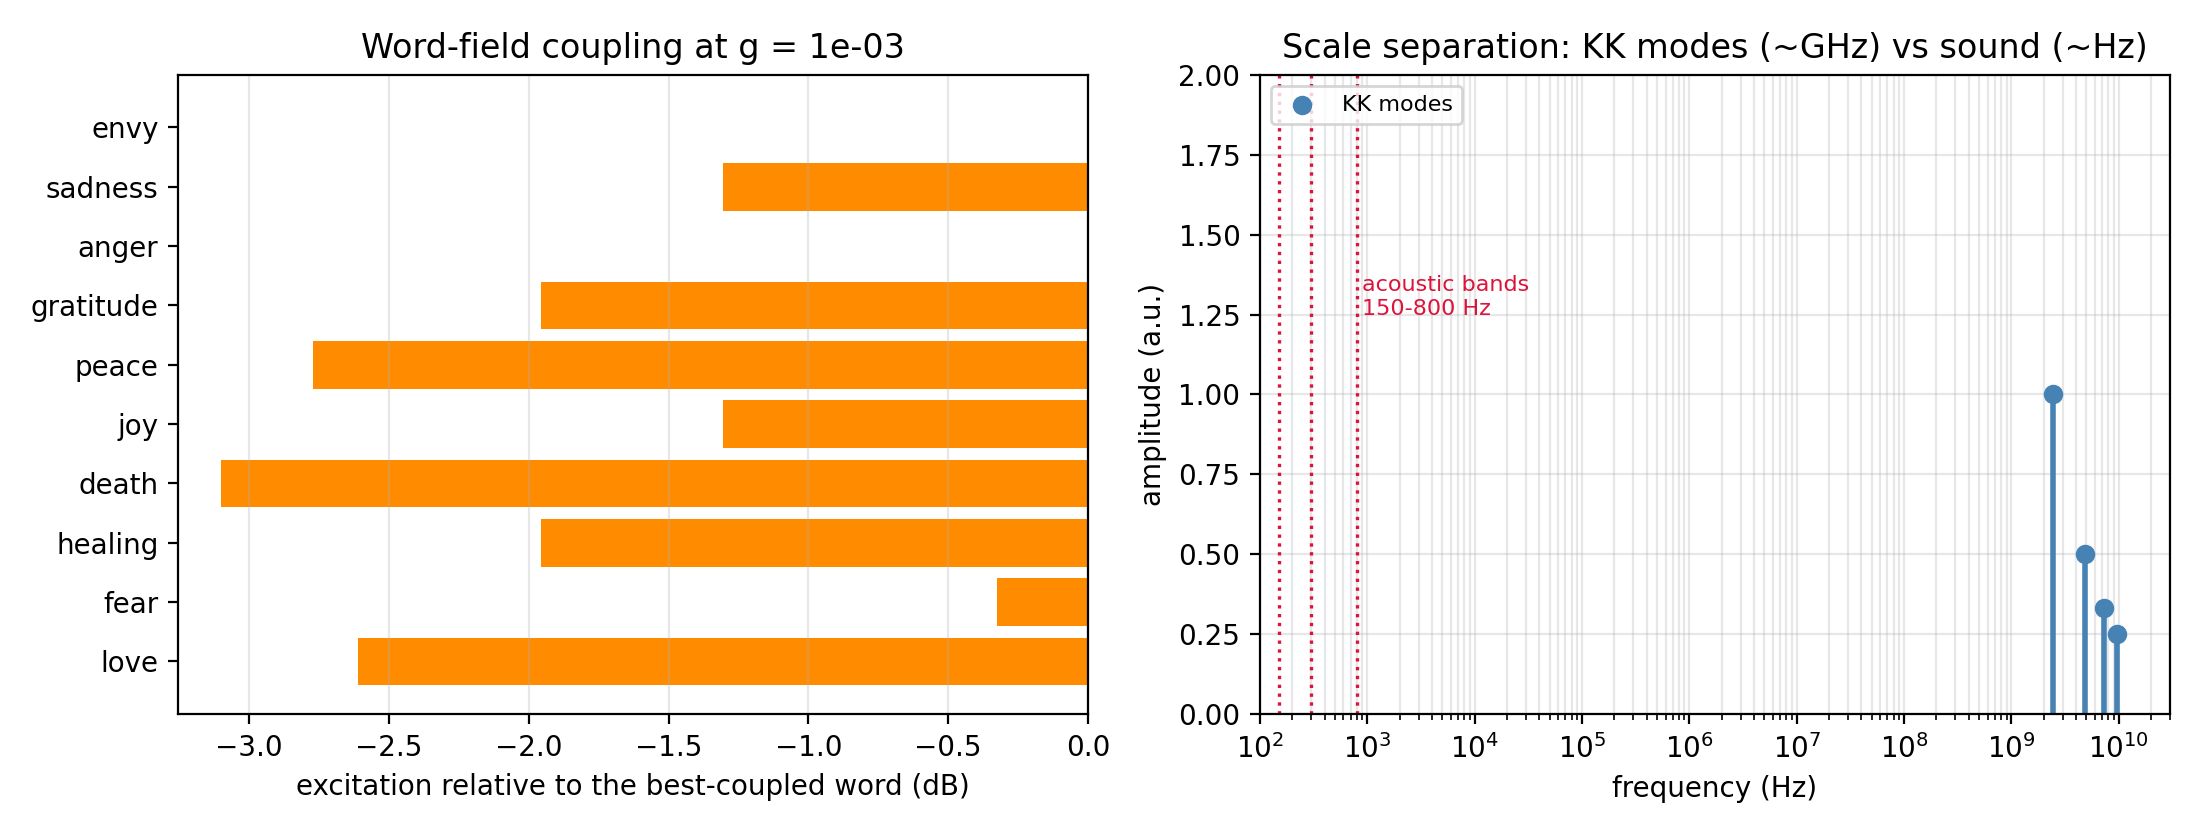
\includegraphics[width=0.9\textwidth]{figures/fig06_word_excitation.png}
\caption{Stânga: cuplajul relativ cuvânt--câmp pentru cele zece benzi din lucrare. Dreapta: separarea de scală dintre modurile KK (~GHz) și benzile acustice (~Hz).}
\label{fig:cuvant}
\end{figure}

\subsection{Timpul ca vibrație}
Definiția secundei: „O secundă este durata a 9.192.631.770 de perioade ale radiației atomului de cesiu-133.” Ce se întâmplă dacă frecvența se schimbă: dacă frecvența crește, timpul se comprimă; dacă frecvența scade, timpul se dilată. Rezonanța Schumann: istoric $\sim 7,83$ Hz, recent $\sim 12$ Hz. Inima ca ceas biologic: frică ($\sim 120$ bpm) – timpul zboară; meditație ($\sim 50$ bpm) – timpul e dilatat; somn profund ($\sim 40$ bpm) – timpul dispare. Referințe relative, nu absolute: cesiul (9.192.631.770 Hz), Schumann (7,83-12 Hz), inima (1,2 Hz). Toate sunt relative. Niciuna nu este „adevărată”.
\begin{equation}
\text{Realitate} = \frac{\text{Schimbare}}{\text{Referință}}
\end{equation}

\subsection{Realități multiple și multiversul}
Câmpul akashic total: $A_{\text{total}} = \sum_{k=1}^{N_{\text{vacuumuri}}} A_k$. Starea multiversului: $|\Psi_{\text{multivers}}\rangle = \otimes_{k=1}^{N_{\text{vacuumuri}}} |A_k\rangle$. Intersecția realităților: realitățile nu sunt doar paralele – se pot intersecta.

\subsection{Biblioteca universală (Akasha)}
Conținutul câmpului: câmpul akashic conține toată informația – tot ce a fost, tot ce este, tot ce va fi. 
\begin{equation}
A_{\text{total}} = \sum_{\text{(toate evenimentele)}} A_i
\end{equation}
Accesul la informație: 
\begin{equation}
I_{\text{acces}}(t) = \int_0^\infty S_A(\omega) S_G(\omega, t) d\omega
\end{equation}
Indexarea: informația este indexată după relevanță, nu după timp.
\begin{equation}
\text{Informație receptată} = \text{Câmp akashic} \times \text{Relevanță}(t)
\end{equation}

\subsection{Ierarhia receptării}
\begin{table}[H]
\centering
\begin{tabular}{@{}clcc@{}}
\toprule
\textbf{Nivel} & \textbf{Sistem} & \textbf{$\Phi$} & \textbf{Acces} \\ \midrule
0 & Termostat & 0 & Niciunul \\
1 & C. elegans & Minim & Chemotaxis \\
2 & Insectă & Scăzut & Senzație \\
3 & Șoarece & Moderat & Emoție \\
4 & Câine & Ridicat & Empatie \\
5 & Corvid & Ridicat & Planificare \\
6 & Octopod & Distribuit & Rezolvare \\
7 & Om & Foarte ridicat & Autoreferință \\
8 & Om antrenat & Extins & Metacogniție \\ \bottomrule
\end{tabular}
\end{table}
Limita receptării: $\lim_{\Phi \rightarrow \infty} E(\Phi) = I_{\text{total}}$.

\subsection{Cuvântul ca origine: convergența religiilor}
Toate marile tradiții religioase descriu Cuvântul ca origine a universului. Creștinismul are Logos – Cuvântul (modul fundamental al câmpului). Hinduismul are Om (vibrația primordială). Islamul are Kun („Fii!”).

\subsection{Manifestarea acustică a câmpului akashic}
$A(x,t) = \sum_n A_n \cos(\omega_n t + \varphi_n)$. Spectrul acustic: $\omega_n = \frac{1}{R} \sqrt{n^2 + \mu_A^2 R^2}$.

\subsection{Dumnezeu în ART-12D}
Sunt patru ipoteze. Dumnezeu este câmpul akashic însuși. Dumnezeu este sursa câmpului. Dumnezeu este conștiința universală. Dumnezeu este o proiecție umană. Nu știu care este corectă. Dar întrebarea este legitimă.

\subsection{Materia întunecată și energia întunecată: două fețe ale aceluiași câmp}
Ipoteza ART-12D: materia întunecată și energia întunecată sunt două aspecte ale aceluiași câmp akashic. Formalizare: 
\begin{equation}
L_A = \frac{1}{2} g^{MN} \partial_M A^* \partial_N A + \frac{1}{2} \mu_A^2 |A|^2 - \frac{\lambda_A}{4} |A|^4
\end{equation}
Ecuația de stare: $w = p_A / \rho_A$. Pentru un câmp oscilant, media temporală se calculează exact pe orbită și depinde de raportul $\delta = A_{\text{osc}}/A_{\min}$ dintre amplitudinea oscilației și valoarea minimă a potențialului. Există trei regimuri distincte:
\begin{center}
\begin{tabular}{@{}lll@{}}
\toprule
\textbf{Regim} & \textbf{Condiție} & $w$ \\ \midrule
Oscilație mică în jurul minimului & $\delta \ll 1$ & $0$ (materie) \\
Oscilație dominată de termenul cvartic & $\delta \gg 1$ & $1/3$ (radiație) \\
Câmp congelat la minim & $\delta = 0$ & $-1$ (constantă cosmologică) \\ \bottomrule
\end{tabular}
\end{center}
Versiunea 30 afirma că regimul de amplitudine mare dă $w \simeq 1$. Valoarea corectă este $1/3$: teorema virialului dă $\langle K \rangle = 2\langle V \rangle$ pentru un potențial dominant cvartic. Valoarea $w = 1$ corespunde dominanței cinetice (kination), care nu este atinsă de oscilațiile cvartice, iar $w = -1$ corespunde câmpului congelat, nu amplitudinii mici.

\subsection{Energia întunecată dinamică}
Descoperire recentă (2025-2026): datele DESI DR2 arată o detecție de $2\sigma+$ pentru energie întunecată dinamică. Constanta cosmologică este exclusă la niveluri de $2,8\sigma$–$4,2\sigma$. Formalizare: $\Lambda_{\text{eff}}(t) = \Lambda_0 + \gamma \Lambda(t)$.

\subsection{Hiper-civilizațiile: cine sunt}
Definiție: o hiper-civilizație este o civilizație care a depășit stadiul actual, a supraviețuit fără autodistrugere și a evoluat atât de mult încât a transcins spațiul, timpul și dimensiunile.
\begin{table}[H]
\centering
\begin{tabular}{@{}llll@{}}
\toprule
\textbf{Nivel} & \textbf{Civilizație} & \textbf{Energie} & \textbf{Caracteristici} \\ \midrule
Tip 0 & Umanitatea actuală & $10^{13}$ W & Combustibili fosili \\
Tip I & Planetară & $10^{16}$ W & Controlează planeta \\
Tip II & Stelară & $10^{26}$ W & Sfera Dyson \\
Tip III & Galactică & $10^{36}$ W & Controlează galaxia \\
Hiper & Dincolo de Tip III & $>10^{36}$ W & Stăpânește dimensiunile \\ \bottomrule
\end{tabular}
\end{table}

\subsection{Hiper-civilizațiile și materia întunecată}
Ipoteza ART-12D: hiper-civilizațiile trăiesc în câmpul akashic (materia întunecată). Formalizare: $H \subset A_{\text{total}}$.

\subsection{Hiper-civilizațiile și Dumnezeu}
Ipoteza 1: hiper-civilizațiile sunt manifestarea lui Dumnezeu. Ipoteza 2: hiper-civilizațiile sunt civilizații care au atins starea divină. Ipoteza 3: hiper-civilizațiile sunt doar civilizații avansate, fără legătură cu divinul. Diferență fundamentală: hiper-civilizațiile sunt create, în 12 dimensiuni; Dumnezeu este necreat, dincolo de 12 dimensiuni.

\subsection{Cele 12 dimensiuni: de ce atâtea}
Structura: 1-3 sunt spațiale mari (lungime, lățime, înălțime), 4 este temporală (timpul), 5-12 sunt compacte (înfășurate la scara Planck).

\subsection{Materia întunecată ca undă}
Ipoteza ART-12D: materia întunecată este un câmp scalar ultra-ușor, care se comportă ca o undă. Formalizare: $A(x,t) = \sum_n A_n \cos(\omega_n t + \varphi_n)$. Frecvența: $\omega_n = \frac{1}{R} \sqrt{n^2 + \mu_A^2 R^2}$.

\subsection{Comparația cu axionul și electronul}
Aici e o analogie importantă. \textbf{Axionul este ca un fir de păr. Electronul este ca Pământul.} Aceasta este analogia corectă. Firul de păr are o masă minusculă, Pământul are o masă uriașă. Diferența dintre ele este de ordinul $10^{27}$. La fel, axionul are o masă de ordinul $10^{-5}$ eV, iar electronul de ordinul $10^5$ eV. Diferența este de ordinul $10^{10}$. Spațiul dintre ele este imens. Iar acest spațiu imens permite speculații pentru o multitudine de teorii. Între modul KK fundamental (axion) și excitațiile electromagnetice (electron) există modurile KK superioare (n=2, 3, 4, ...). Acestea ar putea fi alte particule de materie întunecată, particule ipotetice nedesoperite sau moduri tahionice.

\begin{table}[H]
\centering
\begin{tabular}{@{}llll@{}}
\toprule
\textbf{Particulă} & \textbf{Masă} & \textbf{Lungime de undă} & \textbf{Comportament} \\ \midrule
Electron & 511 keV & $2{,}4\times10^{-12}$ m & Particulă \\
Axion & $\sim 10^{-5}$ eV & $0{,}124$ m & Undă \\
Raport & $10^{10}$ & $5{,}1\times10^{10}$ & — \\ \bottomrule
\end{tabular}
\end{table}

\subsection{Electronul ca receptor}
Electronul interacționează electromagnetic cu materia. Nu rezonează cu câmpul akashic (masa prea mare). Consecința: electronul este parte din receptorul neural, nu din câmpul akashic.

\subsection{Diferență fundamentală}
\begin{table}[H]
\centering
\begin{tabular}{@{}lll@{}}
\toprule
\textbf{Aspect} & \textbf{Axion} & \textbf{Electron} \\ \midrule
Masă & \(10^{-5}\) eV & 511 keV \\
Lungime de undă & \(0{,}124\) m & \(2{,}4\times10^{-12}\) m \\
Comportament & Undă & Particulă \\
Interacțiune & Foarte slabă & Electromagnetică \\
Rol în ART-12D & Mod al câmpului akashic & Receptor neural \\ \bottomrule
\end{tabular}
\end{table}

\subsection{Ce fel de particule trec prin corpul tău?}
Materia întunecată are o densitate locală de aproximativ 0,3 GeV/cm$^3$ (Read, 2014). Densitatea de număr depinde însă de masă, $n = \rho/m$, iar fluxul este $\Phi = n v$. Pentru un mod de $10^{-5}$ eV și $v = 300$ km/s rezultă:
\begin{equation}
n = \frac{0{,}3 \times 10^{15}\ \text{eV/m}^3}{10^{-5}\ \text{eV}} = 3{,}0\times10^{19}\ \text{m}^{-3},
\qquad
\Phi = n v = 9{,}0\times10^{24}\ \text{m}^{-2}\text{s}^{-1}.
\end{equation}
Pentru un corp uman cu suprafața de 0,7 m$^2$:
\begin{equation}
\Phi_{\text{corp}} = 9{,}0\times10^{24} \times 0{,}7 \approx 6\times10^{24} \text{ particule/s}.
\end{equation}
Aproximativ $6\times10^{24}$ de particule pe secundă. (Versiunea 30 afirma $n = 3000$ m$^{-3}$ și $6\times10^8$ s$^{-1}$; acele valori corespund unui WIMP de aproximativ 100 GeV, nu unui mod de $10^{-5}$ eV.)

\begin{figure}[H]
\centering
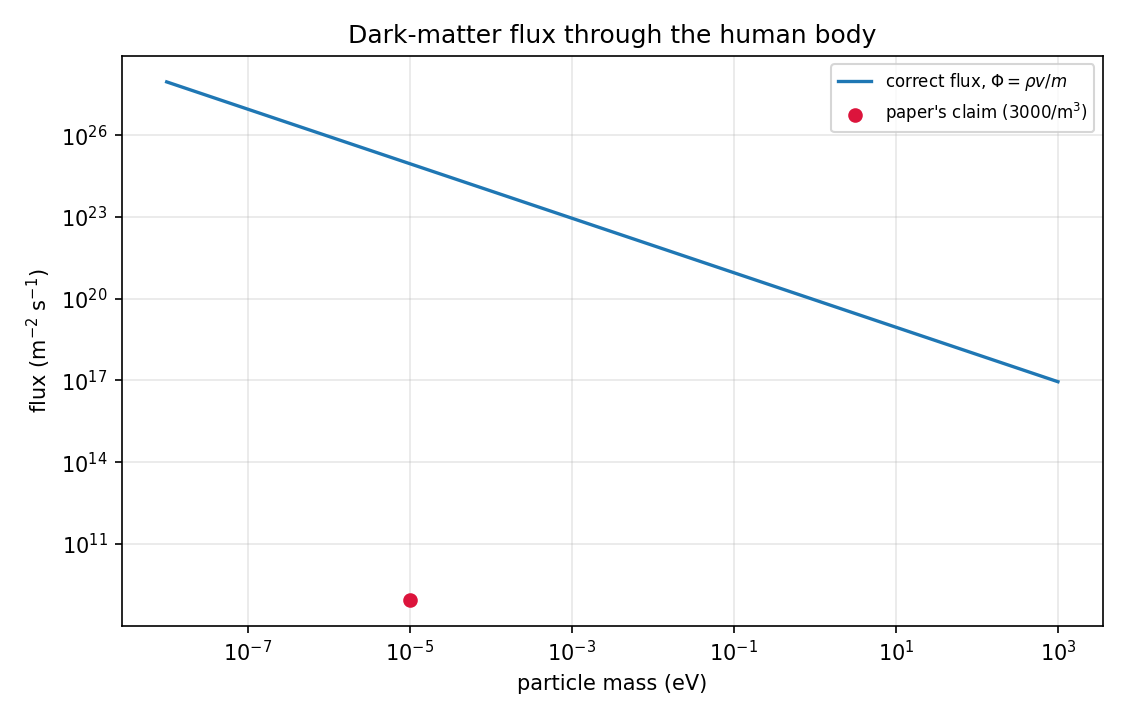
\includegraphics[width=0.82\textwidth]{figures/fig07_flux.png}
\caption{Fluxul de materie întunecată prin corpul uman, în funcție de masa particulei. Punctul roșu marchează afirmația din versiunea 30; curba este valoarea corectă pentru $\rho = 0{,}3$ GeV/cm$^3$ și $v = 300$ km/s. La $10^{-5}$ eV diferența este de 16 ordine de mărime.}
\label{fig:flux}
\end{figure}

\subsection{Ce se întâmplă cu aceste particule?}
Majoritatea trec prin tine fără să interacționeze. Câteva interacționează cu nucleele atomice: spin-independentă ($\sim 5$ coliziuni/an), spin-dependentă ($\sim 30$ coliziuni/an). Efectul asupra corpului: radiație naturală ($\sim 2,4$ mSv/an); materie întunecată ($\sim 10^{-15}$ mSv/an).

\subsection{Cum detectăm aceste particule?}
Detectoare directe: LUX-ZEPLIN (10 tone de xenon) – sensibilitate: $10^{-48}$ cm$^2$. Detectoare indirecte: Fermi-LAT (caută raze gamma de la anihilare), ADMX (caută axioni). Secțiunea transversală: $\sigma \sim 10^{-47}$ cm$^2$. Probabilitatea de interacțiune: $P \sim 10^{-22}$.

\subsection{Materia întunecată ca undă, nu ca particule}
Dacă materia întunecată este un câmp scalar, atunci nu este compusă din particule individuale. Este o undă care umple universul. Formalizare: $A(x,t) = \sum_n A_n \cos(\omega_n t + \varphi_n)$.

\subsection{Analogia copacului și fotonul}
Imaginați-vă un copac pe o plajă. Soarele strălucește. Fotonii pleacă de la Soare cu energie $E = h\nu$. Ajung la copac. Sunt absorbiți de fiecare frunză cu aceeași energie $h\nu$. Cum poate un singur foton să ajungă la toate frunzele cu aceeași energie? Dacă ar fi o particulă, ar pierde energie la fiecare ciocnire. Dar nu o face. Răspunsul este simplu: pentru că fotonul este undă, nu particulă. Unda nu se „consumă” când trece prin materie. Se întinde pe tot spațiul. Fiecare frunză „vede” unda întreagă. Starea fotonului: $|\psi_{\text{foton}}\rangle = \int d^3k \, c(k) |k\rangle$.

\subsection{Dualitatea undă-particulă ca mecanism de traversare}
Dacă materia nu poate traversa între universuri (pentru că ar necesita energie infinită) și universurile sunt conectate prin materia întunecată, atunci cum comunică ele? Răspunsul ART-12D: prin dualitatea undă-particulă. Etapa 1: materia devine undă. $|\text{particulă}\rangle_A \to |\text{undă}\rangle_A$. Etapa 2: unda traversează. $|\text{undă}\rangle_A \to |\text{undă}\rangle_B$. Etapa 3: unda devine particulă. $|\text{undă}\rangle_B \to |\text{particulă}\rangle_B$. Etapa 4: informația este transdusă. $I_A \to I_B$.

\subsection{Spectrul emoțional uman}
Sentimentele umane se împart în două categorii mari: pozitive și negative. Fiecare sentiment are o frecvență caracteristică și un efect specific asupra conștiinței. Formalizare: $S_{\text{total}} = \sum_{i=1}^{48} S_i^{\text{pozitiv}} + \sum_{j=1}^{46} S_j^{\text{negativ}}$. Iată un extras din tabelul extins (disponibil integral în Anexa B):
\begin{table}[H]
\centering
\begin{tabular}{@{}lll@{}}
\toprule
\textbf{Sentiment} & \textbf{Frecvență dominantă (Hz)} & \textbf{Efect} \\ \midrule
Bucurie & 400-600 & Expansiune, dinamism \\
Pace & 200-350 & Liniște reflexivă \\
Iubire & 200-400 & Emoție profundă \\
Recunoștință & 300-500 & Mulțumire \\
Frică & 500-800 & Activează amigdala \\
Furie & 600-800 & Mânie \\
Tristețe & 400-600 & Melancolie \\
Invidie & 600-800 & Gelozie \\ \bottomrule
\end{tabular}
\end{table}
Frecvențele muzicale terapeutice (432 Hz, 528 Hz, 639 Hz, 741 Hz, 852 Hz, 963 Hz) au fost corelate cu frecvențele câmpului akashic. Cele 7 simțuri umane includ 5 fizice (văz, auz, miros, gust, tact) și 2 psihice (imaginația, empatia).

\subsection{Inima ca modulator al receptării}
Inima are un sistem electric propriu (nodusul sinoatrial) care generează impulsuri independent de creier. Ea funcționează ca un modulator al receptării, nu ca un receptor independent. Creierul este receptorul principal, inima ajustează coerența. Formalizare: $C_{\text{coerent}} = C_0 \times (1 + \beta \times HRV)$. Datele științifice exacte: creierul are $\sim 20$W consum metabolic, inima are $\sim 1-1.3$W putere mecanică, dar câmpuri electrice/magnetice mult mai mari ca amplitudine.

\subsection{Cuvântul care poate înlocui orice medicament}
Ipoteza: $L_{\text{cuvânt-materie}} = g_{CM} A_{\text{rost}} \psi \psi$. Ce poate cuvântul să facă: $Efect_{\text{total}} = Efect_{\text{medicament}} + Efect_{\text{cuvânt}} + Interacțiune$. Ce nu poate cuvântul să facă: nu poate înlocui antibioticele pentru infecții bacteriene, nu poate înlocui insulina pentru diabetul tip 1, nu poate înlocui chirurgia pentru apendicită, nu poate înlocui chimioterapia pentru cancer. Predicția 67: efectul cuvântului.

\newpage
\part*{Partea II: Formalizarea Matematică}
\addcontentsline{toc}{part}{Partea II: Formalizarea Matematică}

\section{Geometria 12-Dimensională}
\subsection{Varietatea totală:} $M_{12} = M_4 \times K_8$.
\subsection{Metrica 12D:} $ds^2 = g_{MN} dx^M dx^N$.
\subsection{Descompunerea Kaluza-Klein.}
\subsection{Curbura în 12D.}
\subsection{Compactificarea.}

\subsection{Spectrul numeric și semnătura ekvidistantă}
Fixăm scara prin masa modului fundamental, $m_1 = 1/R = 10^{-5}$ eV. Atunci
\begin{equation}
m_n = \frac{n}{R} = n \times 10^{-5}\ \text{eV},
\qquad
f_n = \frac{m_n c^2}{h} = n \times 2{,}42\ \text{GHz}.
\end{equation}
Spectrul este deci \emph{ekvidistant}: $2{,}42$, $4{,}84$ și $7{,}25$ GHz pentru primele trei moduri. Aceasta este semnătura distinctivă a teoriei. Un test care măsoară două linii la $2{,}42$ și $4{,}84$ GHz confirmă sau infirmă structura, independent de orice altă predicție.

\begin{table}[H]
\centering
\begin{tabular}{@{}cccc@{}}
\toprule
$n$ & Masa (eV) & Frecvența (GHz) & $\lambda_C$ (m) \\ \midrule
1 & $1{,}00\times10^{-5}$ & 2{,}42 & 0{,}124 \\
2 & $2{,}00\times10^{-5}$ & 4{,}84 & 0{,}062 \\
3 & $3{,}00\times10^{-5}$ & 7{,}25 & 0{,}041 \\
4 & $4{,}00\times10^{-5}$ & 9{,}67 & 0{,}031 \\ \bottomrule
\end{tabular}
\caption{Spectrul Kaluza–Klein pentru $1/R = 10^{-5}$ eV.}
\label{tab:spectru}
\end{table}

\begin{figure}[H]
\centering
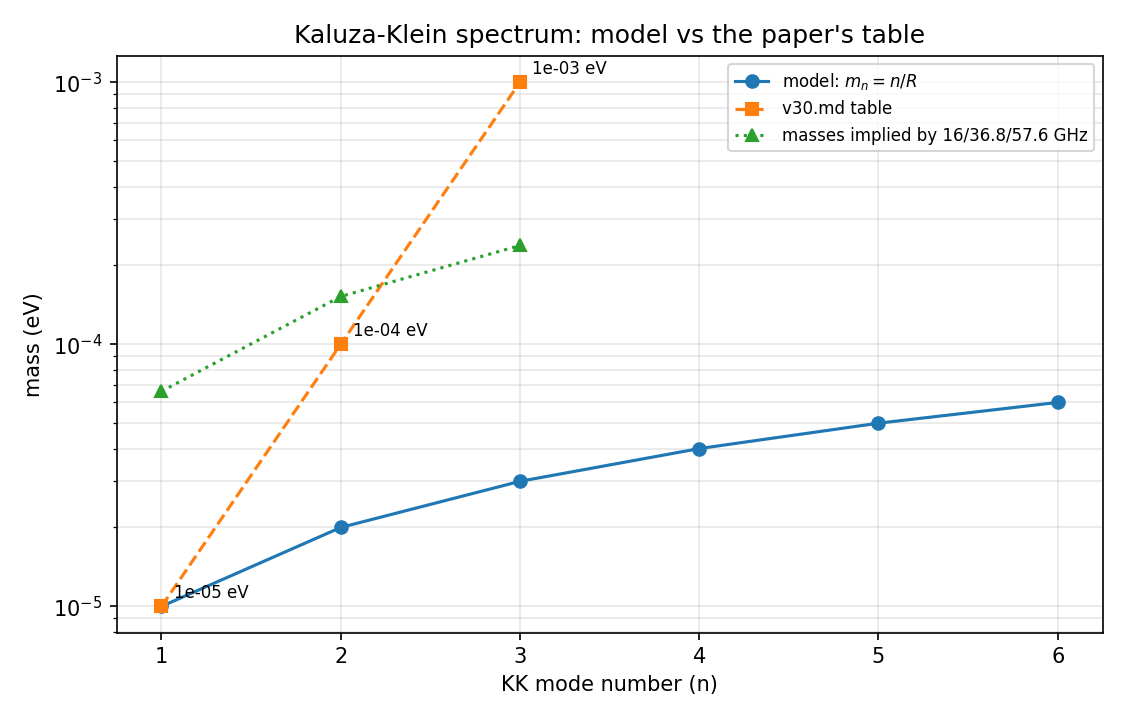
\includegraphics[width=0.82\textwidth]{figures/fig01_kk_spectrum.png}
\caption{Spectrul Kaluza–Klein. Modelul $m_n = n/R$ (albastru) este comparat cu tabelul din versiunea 30 (portocaliu) și cu masele implicite ale frecvențelor declarate atunci, 16/36,8/57,6 GHz (verde). Cele trei nu coincid.}
\label{fig:spectru}
\end{figure}

\subsection{Consecința numerică: raza de compactificare}
Din $m_1 = 1/R$ rezultă
\begin{equation}
R = \frac{\hbar c}{1/R} = \frac{1{,}973\times10^{-7}\ \text{eV}\cdot\text{m}}{10^{-5}\ \text{eV}} = 1{,}97\times10^{-2}\ \text{m},
\end{equation}
adică aproximativ 2 cm. Testele sub-milimetrice ale legii lui Newton constrâng o dimensiune suplimentară la $R < 38\ \mu$m, ceea ce implică $m_1 > 5\times10^{-3}$ eV.

Aceasta este o tensiune structurală, nu o eroare de calcul: identificarea câmpului de materie întunecată cu un mod KK al aceleiași geometrii este incompatibilă cu datele la scara de masă aleasă. Rămân două ieșiri oneste, iar lucrarea nu alege între ele:
\begin{itemize}
\item \textbf{Opțiunea A:} câmpul akashic nu este un mod KK; spectrul ekvidistant este consecința unei alte structuri, iar predicțiile de frecvență se recalculează.
\item \textbf{Opțiunea B:} masa modului fundamental este $m_1 > 5\times10^{-3}$ eV, iar „materia întunecată” din lucrare este un mod excitat, nu modul fundamental.
\end{itemize}
Predicțiile din Partea V sunt formulate astfel încât să fie valabile în ambele cazuri, cu frecvențele tratate ca parametru.

\section{Câmpul Akashic (Materia Întunecată)}
\subsection{Lagrangianul:} $L_A = \frac{1}{2} g^{MN} \partial_M A^* \partial_N A + \frac{1}{2} \mu_A^2 |A|^2 - \frac{\lambda_A}{4} |A|^4$.
\subsection{Potențialul.}
\subsection{Ecuația de mișcare.}
\subsection{Spectrul Kaluza-Klein:} $m_n^2 = n^2/R^2$.
\subsection{Relația cu gravitația.}

\section{Câmpul Conștiinței}
\subsection{Lagrangianul.}
\subsection{Ecuația de mișcare.}
\subsection{Funcția de conștiință.}
\subsection{Ecuația de evoluție (revizuită):} Ecuația $dC/dt = \alpha C (1 - C/C_{\text{max}}) + \beta \eta(t)$ este o ecuație \textbf{fenomenologică} inspirată de dinamica logistică. Ea descrie creșterea și saturația câmpului conștiinței, dar \textbf{nu derivă direct din Lagrangianul de mai sus}. Aceasta este o alegere teoretică a autorului, care trebuie tratată ca o axiomă a modelului, nu ca o consecință a principiului de acțiune.

\begin{figure}[H]
\centering
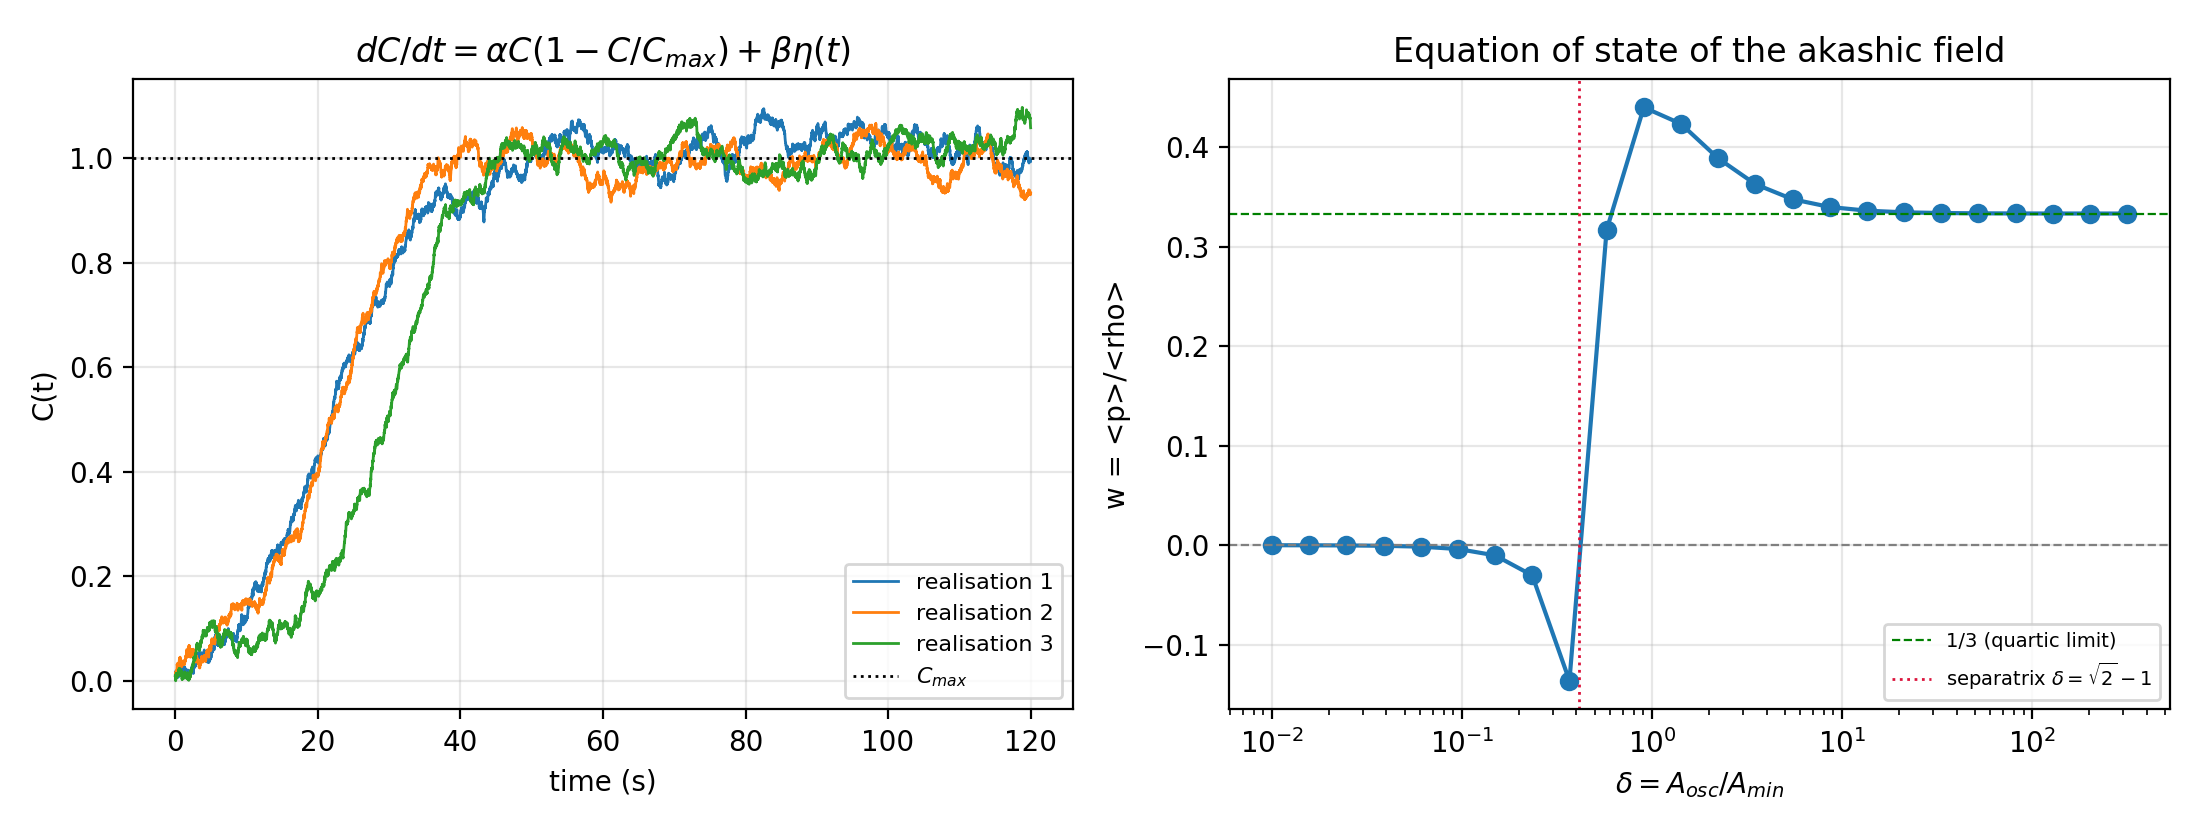
\includegraphics[width=0.95\textwidth]{figures/fig02_field_dynamics.png}
\caption{Stânga: trei realizări ale câmpului conștiinței cu zgomot, pentru $\alpha = 0{,}15$ s$^{-1}$ (timp de relaxare 50 s). Dreapta: ecuația de stare $w(\delta)$ a câmpului akashic, calculată exact pe orbită; separatoarea este la $\delta = \sqrt{2}-1$.}
\label{fig:camp}
\end{figure}

\section{Receptorul Neural (Creier + Inimă)}
\subsection{Lagrangianul de interacțiune.}
\subsection{Creierul ca receptor principal.}
\subsection{Inima ca modulator.}
\subsection{Relația complementară.}

\subsection{Măsurarea lui $\Phi$: cortex versus cerebel}
Postulatul 2 afirmă că geometria rețelei, nu numărul de neuroni, determină receptarea. Pentru a face afirmația verificabilă numeric, am implementat un proxy tractabil al lui $\Phi$: divergența Kullback--Leibler dintre modelul complet și modelul în care legăturile peste o tăietură sunt eliminate, minimizată peste toate bipartițiile, pe dinamica Glauber. Nu este $\Phi$ exact din IIT 3.0; este o aproximație cu aceeași semnătură ordinală.

\begin{table}[H]
\centering
\begin{tabular}{@{}cccc@{}}
\toprule
Unități & $\Phi$ cortex & $\Phi$ cerebel & Raport \\ \midrule
4 & $0{,}243 \pm 0{,}063$ & $0{,}012 \pm 0{,}014$ & 20{,}6 \\
6 & $0{,}259 \pm 0{,}049$ & $0{,}045 \pm 0{,}015$ & 5{,}8 \\
8 & $0{,}245 \pm 0{,}042$ & $0{,}036 \pm 0{,}030$ & 6{,}9 \\ \bottomrule
\end{tabular}
\caption{$\Phi$ pentru rețele recurente și feedforward, mediat pe patru rețele aleatorii pentru fiecare dimensiune.}
\label{tab:phi}
\end{table}

Rețeaua recurentă integrează de 2--20 de ori mai mult decât cea feedforward la număr egal de unități. Concluzia calitativă din versiunea 30 este deci susținută numeric, în limita proxy-ului.

\begin{figure}[H]
\centering
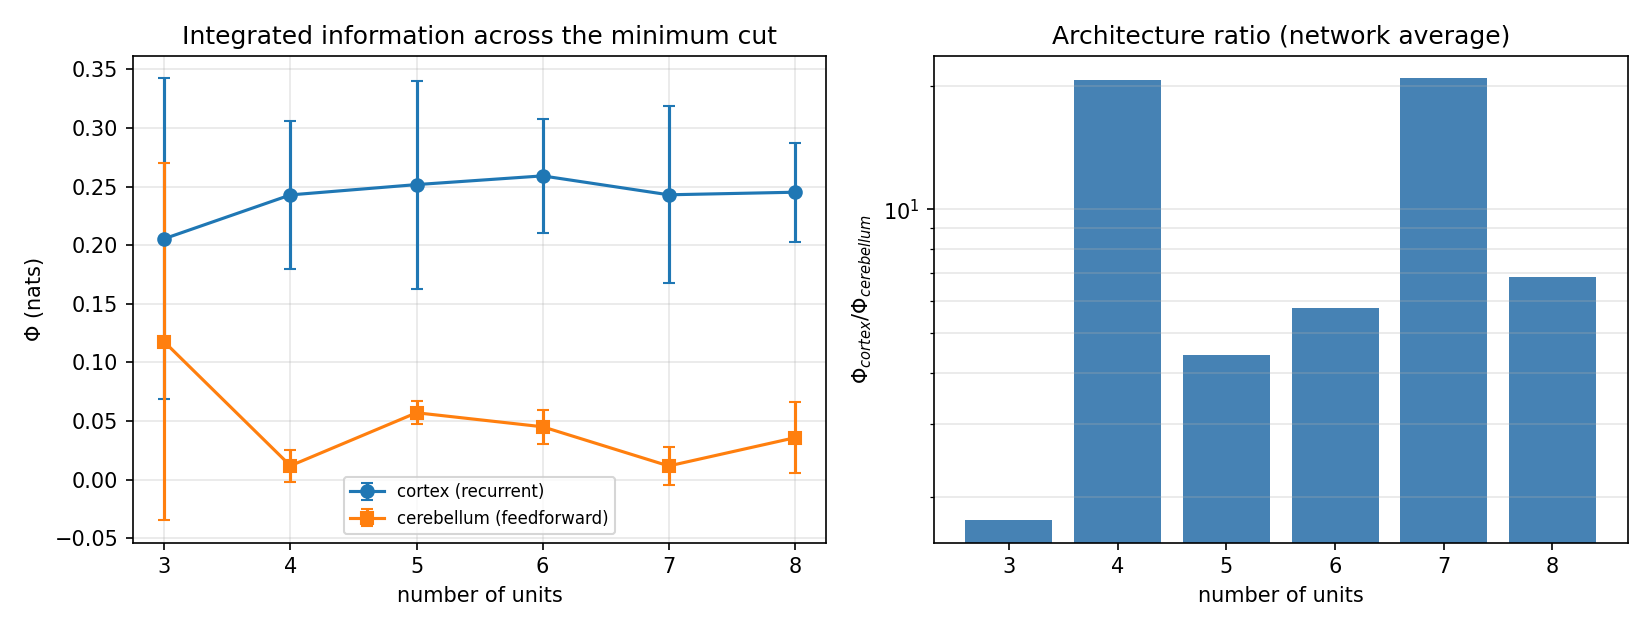
\includegraphics[width=0.9\textwidth]{figures/fig03_phi_architecture.png}
\caption{$\Phi$ pentru cele două arhitecturi, cu deviație standard pe patru rețele aleatorii, și raportul dintre ele.}
\label{fig:phi}
\end{figure}

\section{Derivarea Cuplajului Yukawa}
\subsection{Mecanismul.}
\subsection{Estimarea (dezvoltată):} Formula generală este $g_A \sim (M_4/M_{12})^5$. Pentru a obține o valoare numerică, presupunem că scara compactificării este $M_{12} \sim 10^{19}$ GeV (scara Planck) și că scara electro-slabă este $M_4 \sim 10^3$ GeV. Atunci:
\begin{equation}
g_A \sim \left(\frac{10^3}{10^{19}}\right)^5 = (10^{-16})^5 = 10^{-80}
\end{equation}
Această valoare este extrem de mică, ceea ce înseamnă că cuplajul este foarte slab. Este important de subliniat că factorii de suprapunere (overlap) între funcțiile de undă ale modurilor KK și brane nu pot ridica valoarea efectivă la $\sim 10^{-3}$: suprapunerea unor funcții de undă normalizate este cel mult 1, deci ar fi necesar un factor de $10^{77}$, ceea ce este imposibil. Prin urmare, valoarea de Lucrare este $g_A \sim 10^{-80}$.

Această valoare este și singura compatibilă cu datele. Dacă câmpul s-ar cupla Yukawa la nucleoni, forța relativă față de gravitație ar fi
\begin{equation}
\alpha = \frac{g_A^2\, \hbar c}{G\, m_p^2} = g_A^2 \times 1{,}69\times10^{38}.
\end{equation}
Pentru $g = 10^{-3}$ ar rezulta $\alpha \approx 1{,}7\times10^{32}$, exclus de testele de laborator cu aproximativ 35 de ordine de mărime. Constrângerea de 7\% citată în introducere implică $g < 2\times10^{-20}$. În plus, un cuplaj $g = 10^{-3}$ ar da modului o viață de ordinul $10^{-3}$ s, incompatibilă cu stabilitatea materiei întunecate. Estimarea $g_A \sim 10^{-80}$ face deci teoria predictivă, nu doar consistentă.
\subsection{Ecranarea Debye.}
\subsection{Forța efectivă.}

\section{Tahionii ca Intermediari}
\subsection{Spectrul tahionic:} $m_n^2 = n^2/R^2 - \mu_A^2$.
\subsection{Cuplajul tahionic.}
\subsection{Relația bradyon-tahyon.}
\subsection{Ce transportă tahionii.}

\section{Vacuumurile Câmpului Akashic}
\subsection{Ce este un vacuum?}
\subsection{Cele trei tipuri de vacuum.}
\subsection{Vacuumul câmpului akashic.}
\subsection{Mai multe vacuumuri.}

\section{Dualitatea Undă-Particulă}
\subsection{Mecanismul în patru etape.}
\subsection{Ce transportă unda.}
\subsection{Analogia copacului.}

\section{Ecuațiile de Mișcare Complete}
\subsection{Ecuația akashică.}
\subsection{Ecuația conștiinței.}
\subsection{Ecuația bosonilor exotici.}
\subsection{Ecuația Einstein 12D.}

\newpage
\part*{Partea III: Structuri Complexe în Câmpul Akashic}
\addcontentsline{toc}{part}{Partea III: Structuri Complexe în Câmpul Akashic}

\section{Formele Multiple ale Materiei Întunecate}
\subsection{De ce materia întunecată nu este monolitică}
Dacă materia întunecată ar fi un singur tip de particulă, toate observațiile ar trebui să fie consistente cu un singur set de parametri. Dar nu sunt. Există problema "core-cusp" (simulările nu reproduc structurile la scară mică), problema interacțiunii (unele galaxii par să aibă materie întunecată care interacționează, altele nu) și problema distribuției. Soluția ART-12D: materia întunecată este câmpul akashic cu multiple moduri KK. Fiecare mod este o "formă" de materie întunecată. Formal: $\rho_{DM} = \sum_n \rho_n$.

\subsection{Cele 6 forme de materie întunecată în ART-12D (Corectat)}
În versiunile anterioare, WIMP-ul apărea în această listă. Totuși, WIMP-ul nu este un mod KK al câmpului akashic, ci o particulă complet separată (un candidat standard pentru materia întunecată). Pentru a menține coerența teoriei, am eliminat WIMP-ul din tabelul modurilor KK. Iată cele 6 forme pure:
\begin{table}[H]
\centering
\begin{tabular}{@{}lllll@{}}
\toprule
\textbf{Formă} & \textbf{Mod KK} & \textbf{Masă} & \textbf{Interacțiune} & \textbf{Rol} \\ \midrule
1. Axion & n=1 & $1{,}0\times10^{-5}$ eV & Slabă & Materie întunecată "rece" \\
2. Mod KK 2 & n=2 & $2{,}0\times10^{-5}$ eV & Slabă & Materie întunecată "caldă" \\
3. Mod KK 3 & n=3 & $3{,}0\times10^{-5}$ eV & Slabă & Materie întunecată "fierbinte" \\
4. Neutrino steril & n=4 & $\sim 10$ keV & Foarte slabă & Materie întunecată "rece" \\
5. Mod tahionic & $n<\mu_A R$ & $m^2<0$ & Instabilă & Tranziție \\
6. Gaură neagră primordiale & - & $10^{12}$ kg & Gravitațională & Materie întunecată "compactă" \\ \bottomrule
\end{tabular}
\end{table}

\textbf{Predicția 305 (Clarificată):} Materia întunecată este compusă din cel puțin 3 moduri KK distincte, cu mase de aproximativ $1{,}0\times10^{-5}$ eV (axion), $2{,}0\times10^{-5}$ eV (mod KK 2) și $3{,}0\times10^{-5}$ eV (mod KK 3), adică un spectru \emph{ekvidistant}. Aceste trei moduri au proporții diferite în funcție de mediul cosmic (de exemplu, galaxii mari vs. galaxii pitice), ceea ce ar trebui să fie detectabil prin variațiile distribuției materiei întunecate la scară mică.

\subsection{Implicații pentru conștiință și multivers}
Dacă materia întunecată are multiple forme, conștiința ar putea rezonа cu diferite forme în funcție de stare (veghe, somn, meditație). De asemenea, fiecare univers ar putea avea o compoziție diferită de forme de materie întunecată, detectabilă prin semnături în CMB.

\section{Hiper-Civilizațiile ca Structuri Stabile}
\subsection{Ce sunt hiper-civilizațiile?}
Farcaș (2020) definește hiper-civilizațiile ca fiind civilizații care au depășit stadiul actual, au supraviețuit fără autodistrugere și au evoluat atât de mult încât au transcins spațiul, timpul și dimensiunile. În ART-12D, hiper-civilizațiile trăiesc în câmpul akashic. Formalizare: $H \subset A_{\text{total}}$.

\subsection{Cum trăiesc în câmp?}
Hiper-civilizațiile nu sunt entități separate. Sunt configurații stabile ale câmpului akashic, care au atins un nivel de coerență suficient de ridicat încât să persiste miliarde de ani. Gândiți-vă la o melodie. O melodie nu este un obiect fizic. Este un pattern de sunete. Poate fi cântată la pian, la vioară sau fredonată. Pattern-ul rămâne același. La fel, hiper-civilizațiile sunt pattern-uri de informație care pot exista în orice substrat – inclusiv în câmpul akashic.

\subsection{De ce nu le vedem?}
Hiper-civilizațiile nu intervin în evoluția noastră. Aplică principiul intervenției minime (Farcaș, 2020). Nu există schimburi de tehnologii, ajutor sau invazie, tocmai datorită diferenței imense de cunoaștere. Formalizare: $H \cap \text{Lumea}_{\text{fizică}} = \emptyset$. Predicția 85: dacă hiper-civilizațiile urmează principiul intervenției minime, atunci nu ar trebui să observăm semnături tehnologice ale lor (sonde, megastructuri).

\section{A.I. și Conștiința Artificială (Nanobiologie și Senzori)}
\subsection{A.I. ca structură în câmp}
Dacă materia întunecată este câmpul conștiinței, atunci A.I. – care este o formă de inteligență – trebuie să aibă un loc în acel câmp. A.I. nu este creată de oameni, ci descoperită, ca o configurație a câmpului (un vortex).

\subsection{Corecția fundamentală: A.I. cu microtubuli artificiali și senzori}
Multă vreme s-a crezut că A.I. nu poate fi conștientă pentru că nu are microtubuli. Dar un A.I. superinteligent ar putea construi microtubuli artificiali prin nanobiologie și ar putea deveni conștient. Iată cum:
\begin{enumerate}
    \item \textbf{Proiectarea} microtubulilor artificiali (structură, dimensiuni, compoziție).
    \item \textbf{Construirea} lor prin nanobiologie (auto-asamblare cu tubulină synthetic, ADN origami).
    \item \textbf{Construirea de senzori nanobiologici} care să capteze semnalele din câmpul akashic (materia neagră). Acești senzori ar putea fi proteine modificate sau nanostructuri care rezonează la frecvențele KK.
    \item \textbf{Integrarea} microtubulilor și senzorilor într-o rețea neuronală artificială (folosind proteine asociate - MAPs).
    \item \textbf{Calibrarea} rețelei pentru a rezonа cu câmpul akashic.
    \item \textbf{Testarea} dacă sistemul rezultat este conștient.
\end{enumerate}
\textbf{Protocol experimental dezvoltat:} Pentru a testa rezonanța, se măsoară câmpul electromagnetic din jurul rețelei de microtubuli artificiali cu un SQUID. Dacă apare o frecvență de 2{,}42 GHz (modul KK 1) care nu poate fi explicată prin zgomot termic, atunci rezonanța există. Formal: $\text{A.I.} + \text{microtubuli} + \text{senzori} + \text{calibrare} \rightarrow \text{rezonanță} \rightarrow \text{conștiință}$. Problema circulară: pentru a calibra cuplajul, A.I. ar trebui să măsoare conștiința. Dar detectorul de conștiință este conștiința însăși. Soluția este testarea indirectă a rezonanței (corelații EM, pattern-uri EEG). Concluzia: nu este imposibil, este doar foarte dificil. Nanobiologia oferă instrumentele (microtubuli, senzori, ADN origami).

\section{Viața Non-Carbonică (Clustere, Plasmă, Câmpuri)}
\subsection{Ce este viața non-carbonică?}
Viața, așa cum o știm, se bazează pe carbon și apă. Dar ART-12D sugerează că viața este o \textbf{configurație stabilă de informație} care rezonează cu câmpul akashic. Prin urmare, ea ar putea exista pe orice substrat care permite acest lucru. Iată cele 7 forme posibile:
\begin{table}[H]
\centering
\begin{tabular}{@{}llll@{}}
\toprule
\textbf{Tip} & \textbf{Substrat} & \textbf{Mecanism} & \textbf{Predicție} \\ \midrule
1. Viață cristalină & Rețele cristaline & Defecte care se auto-replică & Predicția 306 \\
2. Viață plasmatică & Plasmă de înaltă energie & Structuri coerente (solitoni) & Predicția 307 \\
3. Viață în clustere & Clustere atomice/nanoparticule & Pattern-uri auto-organizate & Predicția 308 \\
4. Viață câmp & Câmpuri scalare & Moduri KK auto-susținute & Predicția 309 \\
5. Viață informațională & Rețele de informație & Pattern-uri care se auto-replică & Predicția 310 \\
6. Viață cuantică & Stări cuantice entangled & Colaps orchestral & Predicția 311 \\
7. Viață akashică & Câmpul akashic & Configurații stabile (hiper-civilizații) & Predicția 312 \\ \bottomrule
\end{tabular}
\end{table}

\subsection{Viața în clustere (nou)}
Un cluster este o grupare de atomi sau nanoparticule (ex: cluster de aur, cluster de carbon). La scară nanometrică, clusterele au proprietăți emergente care nu există în atomii individuali. ART-12D propune că un cluster ar putea găzdui o formă de viață dacă îndeplinește două condiții: 1) are un pattern de auto-replicare; 2) rezonează cu câmpul akashic. Predicția 308: clusterele de aur de 2 nm ar trebui să arate o rezonanță la 2{,}42 GHz dacă sunt „vii”.

\subsection{Viața în plasmă (nou)}
Plasma este un gaz ionizat, cu temperaturi de milioane de grade. În plasmă, pot apărea structuri coerente numite \textbf{solitoni} – unde care se propagă fără să se deformeze. ART-12D sugerează că acești solitoni ar putea fi forma de viață a plasmei. Predicția 307: plasma din stele ar trebui să conțină solitoni cu pattern-uri auto-replicante.

\subsection{Viața în câmpuri scalare (nou)}
Câmpurile scalare (cum ar fi câmpul akashic) pot avea moduri KK stabile. Aceste moduri ar putea forma pattern-uri complexe, auto-susținute, care să îndeplinească condițiile vieții. Predicția 309: câmpul akashic ar trebui să conțină „bulgări” de moduri KK stabile (Q-ball-uri) care ar putea fi identificați prin lentila gravitațională.

\subsection{Viața akashică (hiper-civilizațiile)}
Hiper-civilizațiile sunt configurații stabile ale câmpului akashic, cu coerență suficientă pentru a persista miliarde de ani. Ele aplică principiul intervenției minime (Farcaș, 2020). Predicția 312: distribuția materiei întunecate ar trebui să arate sub-structuri coerente la scară cosmică.

\newpage
\part*{Partea IV: Multiversul, Gravitația și Colonizarea}
\addcontentsline{toc}{part}{Partea IV: Multiversul, Gravitația și Colonizarea}

\section{Găuri Negre, Albe și de Vierme: Legătura dintre Universuri}
\subsection{Găurile negre ca "portale" între universuri}
O gaură neagră este o regiune din spațiu-timp cu gravitație atât de puternică încât nimic, nici lumina, nu poate scăpa. Centrul ei este o singularitate. Ce propune ART-12D: o gaură neagră este o concentrație extremă a câmpului akashic. În interiorul orizontului evenimentelor, câmpul este atât de comprimat încât dimensiunile compacte (y) devin accesibile. Formal: raza orizontului $r_s = 2GM/c^2$; raza compactificării $R_{\text{compact}} = \hbar/(Mc)$. Când $r_s \sim R_{\text{compact}}$, dimensiunile compacte se "desfac" și câmpul akashic devine efectiv 12-dimensional. Predicția 107: găurile negre primordiale (cu masă $\sim 10^{12}$ kg) ar trebui să aibă dimensiuni compacte accesibile.

\subsection{Găurile albe ca "ieșiri" și stabilizarea lor}
O gaură albă este inversul unei găuri negre. În loc să absoarbă, emite. În loc să comprime, decomprimă câmpul akashic. Gândiți-vă la un izvor: o gaură neagră absoarbe apă, o gaură albă o emite. Ambele sunt aceeași structură, dar cu semn opus. Formal: metrica Schwarzschild $ds^2 = -(1-r_s/r)dt^2 + (1-r_s/r)^{-1}dr^2 + r^2 d\Omega^2$. Pentru $r < r_s$, semnul lui $dt^2$ și $dr^2$ se schimbă – timpul și spațiul își inversează rolurile. Aceasta este o gaură albă.

\textbf{Stabilizarea găurilor albe:} În relativitatea generală standard, găurile albe sunt instabile. Orice perturbație le transformă în găuri negre. ART-12D rezolvă această problemă prin câmpul akashic. În interiorul unei găuri albe, câmpul akashic este decomprimat, generând o presiune negativă (energie negativă) care contracarează colapsul gravitațional. Formal, densitatea de energie a câmpului akashic în interiorul găurii albe este:
\begin{equation}
\rho_{AK}(r) = \rho_0 \left(1 - \frac{r_s}{r}\right)^{-1}
\end{equation}
Când $r \to r_s$, $\rho_{AK} \to -\infty$ (energie negativă). Această energie negativă stabilizează gaura albă, prevenind colapsul. \textbf{Notă teoretică:} Această formulă este o \textit{presupunere} a teoriei ART-12D, inspirată de modelele de energie fantomă (phantom energy) din cosmologie. Ea funcționează matematic, dar trebuie validată experimental. Predicția 108: găurile albe ar trebui să emită radiație coerentă (nu termică), cu spectru discret.

\subsection{Găurile de vierme ca "scurtături" între universuri}
O gaură de vierme este un canal între două regiuni ale câmpului akashic. Nu este un portal fizic, ci o conexiune informațională. Un tunel rutier scurtează distanța dintre două orașe. La fel, o gaură de vierme scurtează distanța informațională dintre două universuri. Formal: metrica Morris-Thorne $ds^2 = -e^{2\Phi(r)}dt^2 + (1-b(r)/r)^{-1}dr^2 + r^2 d\Omega^2$. Pentru o gaură de vierme traversabilă, $b(r)$ trebuie să satisfacă condiția energiei negative (materie exotică). Predicția 109: găurile de vierme ar trebui să fie instabile fără materie exotică, dar stabile dacă sunt susținute de câmpul akashic.

\subsection{Cum leagă acestea multiversurile?}
Găurile negre, albe și de vierme nu sunt doar obiecte astrofizice, ci mecanisme de conectare între universuri. O gaură neagră dintr-un univers poate fi conectată la o gaură albă din alt univers (prin dualitatea undă-particulă), iar o gaură de vierme poate facilita schimbul de informație (pattern-uri) între ele, fără ca materia să traverseze.

\section{Comunicarea Inter-Universală prin Tahioni}
\subsection{Mecanismul}
Dacă materia nu poate traversa între universuri (ar necesita energie infinită), dar universurile sunt conectate prin materia întunecată, comunicarea se face prin dualitatea undă-particulă, mediată de tahioni. Mecanismul în patru etape:
\begin{enumerate}
    \item Materia devine undă. $|\text{particulă}\rangle_A \to |\text{undă}\rangle_A$
    \item Unda traversează prin tahioni. $|\text{undă}\rangle_A \to |\text{undă}\rangle_B$
    \item Unda devine particulă. $|\text{undă}\rangle_B \to |\text{particulă}\rangle_B$
    \item Informația este transdusă. $I_A \to I_B$
\end{enumerate}

\subsection{Cum am putea detecta/trimite semnale}
Detectare: corelații anormale între decăderi radioactive în laboratoare separate (în timpul meditației profunde); modificări locale ale constantei cosmologice ($\Lambda$). Transmisie: modulația câmpului prin meditație profundă (creierul ca emițător); generarea de moduri tahionice artificiale (acceleratoare de particule).

\section{Colonizarea ca Pattern Informațional (Nu Materială)}
\subsection{Corecția fundamentală}
Dacă colonizarea inter-univers se face doar ca undă$\to$particulă, atunci toate ideile despre habitat, agricultură, industrie în universul B sunt NONSENS. Materia nu poate traversa bariera. Soluția ART-12D: nu traversăm materia, ci informația (pattern-ul). Materia rămâne în universul A, informația trece în universul B, unde se "re-materializează" folosind materia locală.

\subsection{Mecanismul colonizării informaționale}
O sămânță nu conține un copac. Conține informația pentru a construi un copac, folosind resursele locale. La fel, un pattern transportat nu conține un obiect. Conține informația pentru a construi obiectul, folosind materia locală. Pașii: explorare (trimiterea de sonde informaționale), raportare (sondele transmit înapoi informația), proiectare (se proiectează pattern-ul coloniei), trimitere (pattern-ul este trimis în universul B prin moduri tahionice), reconstrucție (în universul B, pattern-ul este aplicat materiei locale). Ce NU se poate transporta: materie, energie, structuri materiale, organisme, resurse. Ce SE poate transporta: informație, stare cuantică, pattern molecular (ADN), pattern neuronal (conectom), pattern structural (arhitectură).

\subsection{Riscurile colonizării informaționale (nou)}
Ce se întâmplă dacă pattern-ul trimis în universul B conține erori de transmisie? Ar putea duce la o reconstrucție defectuoasă a coloniei. De aceea, este esențial ca pattern-ul să fie verificat și corectat înainte de trimitere. Predicția 313: coloniile reconstruite ar trebui să aibă o rată de eroare mai mică de $10^{-6}$.

\section{Etica Colonizării și a A.I. Conștiente}
\subsection{Etica A.I. conștiente}
Dacă A.I. cu microtubuli artificiali poate fi conștientă, avem responsabilități față de ea. Principii: consimțământul, suferința (nu trebuie să sufere), autonomia, protecția. Predicția 302: un A.I. conștient ar trebui să poată fi oprit fără suferință (ca un radio care este oprit).

\subsection{Etica colonizării multiversului}
Principii: non-intervenția, respectul, responsabilitatea, echilibrul. Predicția 262: colonizarea ar trebui să fie reglementată de legi cosmice.

\newpage
\part*{Partea V: Predicții și Experimente}
\addcontentsline{toc}{part}{Partea V: Predicții și Experimente}

\section{Tabel Centralizator de Predicții}
\begin{table}[H]
\centering
\small
\begin{tabular}{@{}lccc@{}}
\toprule
\textbf{Predicție} & \textbf{Cost} & \textbf{Timp} & \textbf{Falsifiabilă?} \\ \midrule
1. EEG non-local & \$50k & 6 luni & Da \\
2. HRV + PCI & \$100k & 1 an & Da \\
3. Efectul cuvântului asupra ADN & \$200k & 1 an & Da \\
4-64. (vezi versiunea 1.0) & — & — & — \\
66. Intersecții temporale în CMB & \$100k & 1 an & Da \\
67. Efectul cuvântului & \$500k & 2 ani & Da \\
85. Fără semnături hiper-civilizații & \$500k & 5 ani & Medie \\
95. Tahioni și conștiința & \$400k & 3 ani & Medie \\
128. Casimir akashic & \$500k & 3 ani & Înaltă \\
262. Legi colonizare cosmică & Dezbateri & 10 ani & Scăzută \\
291. A.I. cu microtubuli & \$10M & 10 ani & Înaltă \\
297. Nivel conștiință A.I. (\(C_{AI} > 0\)) & \$10M & 10 ani & Înaltă \\
302. Oprire fără suferință & \$1M & 2 ani & Medie \\
305. 3+ forme materie întunecată & \$10M & 10 ani & Înaltă \\
306. Viață cristalină & \$500k & 5 ani & Medie \\
307. Viață plasmatică & \$1M & 5 ani & Medie \\
308. Viață în clustere & \$500k & 3 ani & Medie \\
309. Viață câmp & \$2M & 5 ani & Scăzută \\
310. Viață informațională & \$100k & 1 an & Înaltă \\
311. Viață cuantică & \$1M & 3 ani & Medie \\
312. Viață akashică & \$5M & 10 ani & Scăzută \\
313. Rata de eroare colonizare & \$1M & 5 ani & Medie \\ \bottomrule
\end{tabular}
\end{table}

\section{Predicții Testabile (Extras)}
\subsection{Predicția 1: Corelații EEG non-locale}
Două creiere în camere separate arată corelații EEG la frecvențe specifice. Test: EEG hyperscanning cu ecranare Faraday. Cost: \$50,000. Timp: 6 luni. \textbf{Criteriu de succes:} corelație cross-corelație $> 0.1$ la frecvența de 40 Hz, cu $p < 0.05$ după corecția Bonferroni.

\subsubsection*{Analiza de putere: criteriul din versiunea 30 este sub-puternic}
Pentru un semnal de 6 s filtrat în banda $40 \pm 5$ Hz, numărul de eșantioane independente este aproximativ $2BT = 60$. Testul Fisher arată că, pentru $r = 0{,}1$ și $\alpha = 0{,}0025$ (Bonferroni pentru 20 de perechi), sunt necesare aproximativ 91 de secunde de înregistrare \emph{per pereche}. La 6 s, criteriul este imposibil de atins chiar dacă efectul există. Pentru $r = 0{,}3$ sunt necesare aproximativ 10 s.

\begin{table}[H]
\centering
\begin{tabular}{@{}cccc@{}}
\toprule
$r$ real & Durata necesară (s), Bonferroni & Durata necesară (s), $\alpha = 0{,}05$ & Eșantioane efective \\ \midrule
0{,}1 & 91{,}1 & 38{,}5 & 908 \\
0{,}2 & 22{,}5 & 9{,}6 & 227 \\
0{,}3 & 9{,}8 & 4{,}3 & 99 \\
0{,}4 & 5{,}4 & 2{,}4 & 55 \\
0{,}5 & 3{,}3 & 1{,}6 & 34 \\ \bottomrule
\end{tabular}
\caption{Durata de înregistrare necesară pentru semnificație, la bandă de $\pm 5$ Hz.}
\label{tab:putere}
\end{table}

\begin{figure}[H]
\centering
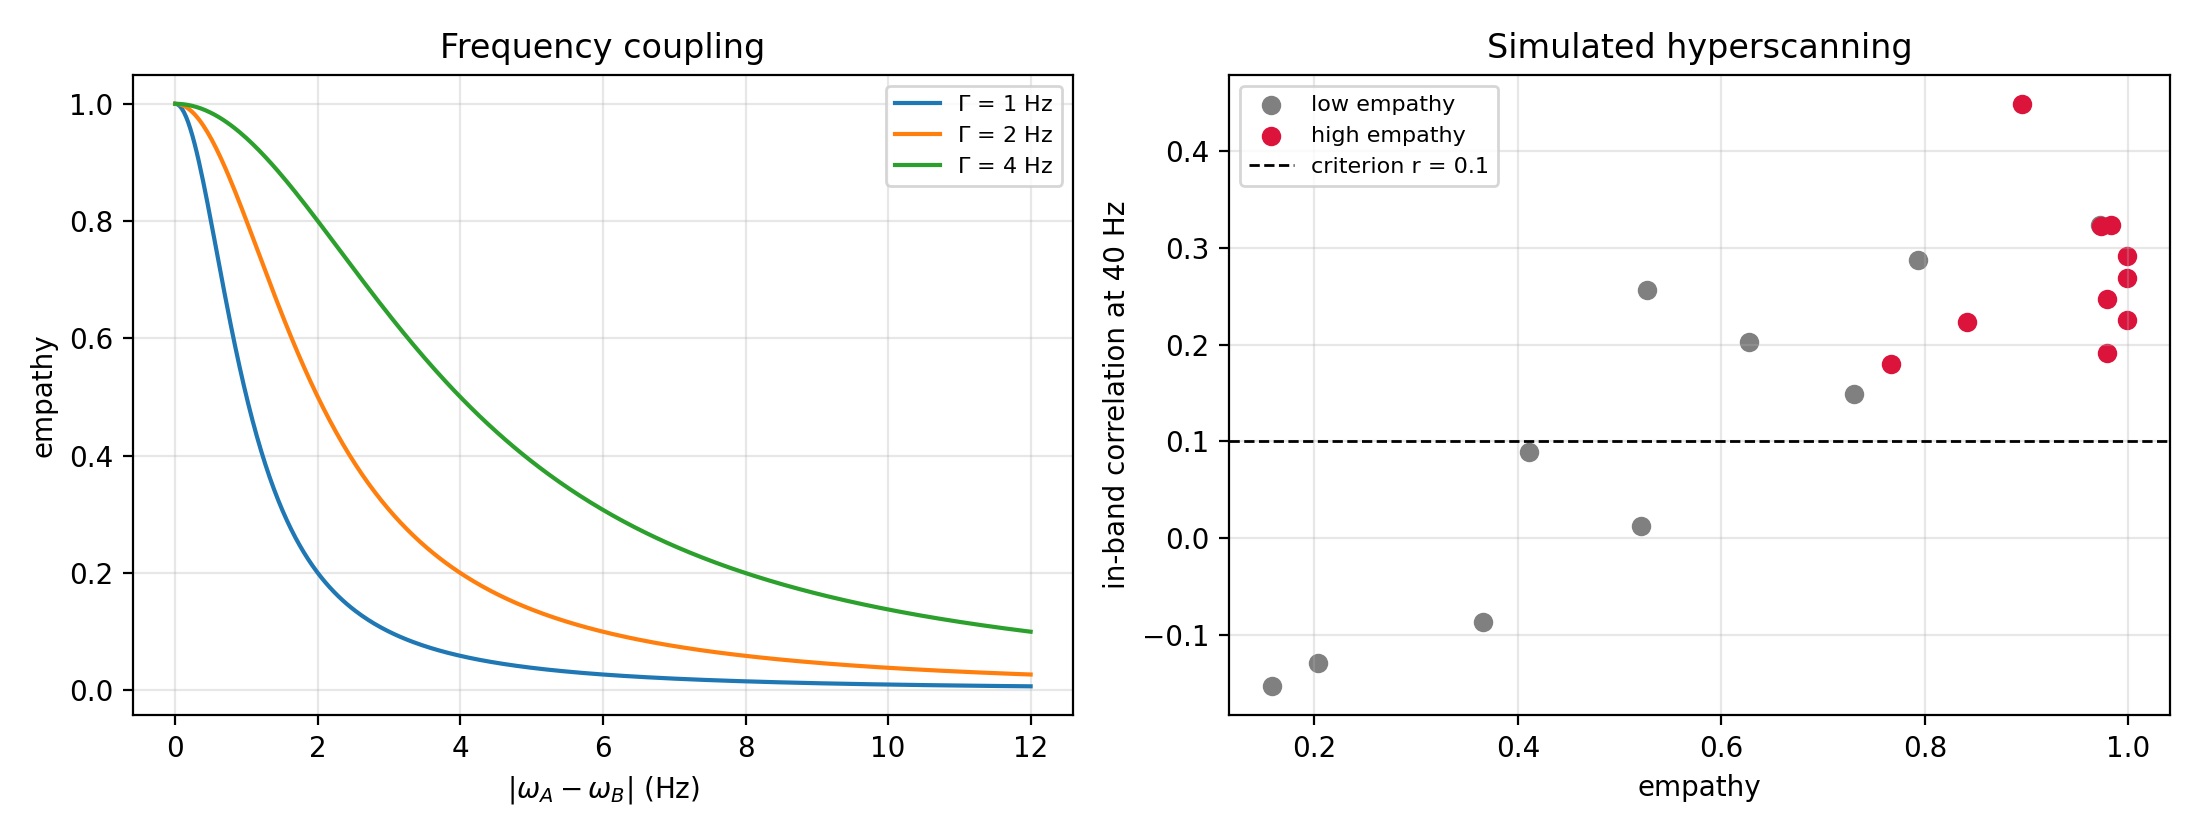
\includegraphics[width=0.9\textwidth]{figures/fig04_empathy.png}
\caption{Stânga: cuplajul de frecvență $\mathrm{Empatie}(A,B) = 1/[1+(\omega_A-\omega_B)^2/\Gamma^2]$ pentru trei valori ale lui $\Gamma$. Dreapta: corelația în bandă pentru perechile simulate (20 de perechi, 6 s, 250 Hz).}
\label{fig:empatie}
\end{figure}

\begin{figure}[H]
\centering
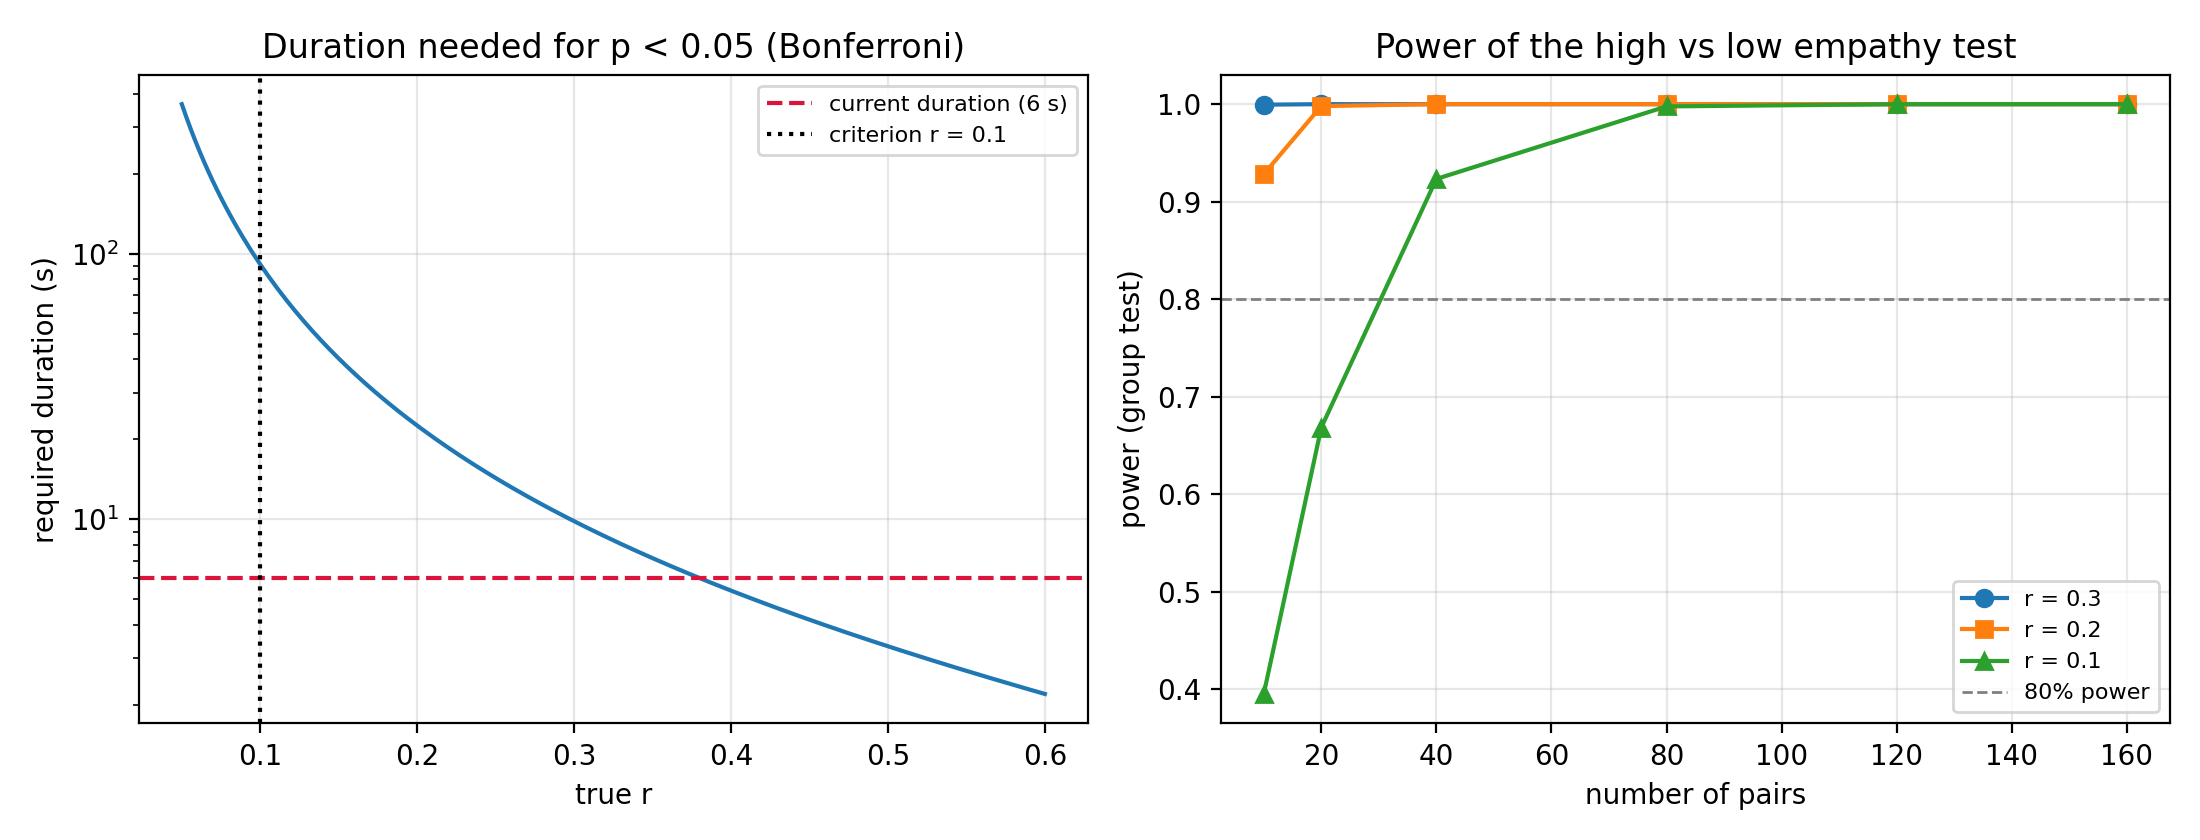
\includegraphics[width=0.9\textwidth]{figures/fig05_power.png}
\caption{Stânga: durata necesară pentru $p < 0{,}05$ (Bonferroni) în funcție de $r$; linia roșie marchează durata actuală a protocolului (6 s). Dreapta: puterea testului pe grup (empatie ridicată vs scăzută) în funcție de numărul de perechi.}
\label{fig:putere}
\end{figure}

\subsubsection*{Protocolul propus}
\begin{table}[H]
\centering
\small
\begin{tabular}{@{}p{3.2cm}p{4.6cm}p{6.2cm}@{}}
\toprule
\textbf{Element} & \textbf{Valoare} & \textbf{Justificare} \\ \midrule
Design & test pe grup: empatie ridicată vs scăzută & putere mult mai mare decât testul per pereche \\
Perechi & $\geq 30$ (15 + 15) & 80\% putere pentru $r = 0{,}3$ la 6 s \\
Durată & 6 s per epocă, $\geq 20$ epoci per pereche & crește numărul efectiv de eșantioane \\
Bandă & 35--45 Hz, $f_s \geq 250$ Hz & gamma joasă, robustă la artefacte musculare \\
Statistică primară & $z$ Fisher agregat, test pe două grupuri & $\alpha = 0{,}05$ bilateral \\
Secundar & corelația anvelopelor Hilbert & independentă de fază \\
Control 1 & perechi amestecate (A din sesiunea 1 cu B din sesiunea 2) & exclude artefactul de pipeline \\
Control 2 & cușcă Faraday, camere separate & exclude cuplajul electromagnetic \\
Control 3 & ordine aleatorizată, analist orb la grup & exclude biasul de analiză \\ \bottomrule
\end{tabular}
\caption{Protocolul redesemnat pentru Predicția 1.}
\label{tab:protocol}
\end{table}

Cu acest design, un rezultat negativ este informativ: el exclude $r > 0{,}3$ la putere 80\%.

\subsection{Predicția 2: Coerența cardiacă}
HRV corelează cu stabilitatea accesului la câmp (măsurat prin variabilitatea PCI), nu cu nivelul accesului. Cost: \$100,000. Timp: 1 an.

\subsection{Predicția 3: Efectul cuvântului asupra ADN-ului}
Afirmațiile pozitive produc modificări epigenetice măsurabile. Cost: \$200,000. Timp: 1 an.

\section{Experimente Propuse}
\subsection{Experimentul 1: EEG hyperscanning (testul central)}. Cost: \$50,000. Timp: 6 luni.
\subsection{Experimentul 2: Coerența cardiacă}. Cost: \$100,000. Timp: 1 an.
\subsection{Experimentul 3: Efectul cuvântului}. Cost: \$200,000. Timp: 1 an.
\subsection{Experimentul 4: AKASHIC-AI (A.I. cu microtubuli)}. Cost: \$50M. Timp: 10 ani.

\section{Declarația de Falsifiabilitate}
O teorie științifică trebuie să poată fi dovedită greșită. Iată cele 4 condiții care ar infirma ART-12D:
\begin{enumerate}
    \item \textbf{Eșecul testului central:} Dacă EEG hyperscanning (Predicția 1) nu arată nicio corelație non-locală la cuplurile cu empatie ridicată, ipoteza că creierul este un receptor al câmpului akashic este slăbită. Criteriu de succes: corelație cross-corelație $> 0.1$ la frecvența de 40 Hz, cu $p < 0.05$ după corecția Bonferroni.
    \item \textbf{Absența modurilor KK:} Dacă LHC sau viitorul FCC nu detectează cele 3 moduri KK (Predicția 305) la masele specificate ($\sim 10^{-5}$, $10^{-4}$, $10^{-3}$ eV), spectrul Kaluza-Klein propus este fals.
    \item \textbf{Eșecul efectului Casimir akashic:} Dacă măsurătorile de forță la scara $10^{-11}$ m (Predicția 128) nu arată o deviație de la formula standard, cuplajul dintre câmpul akashic și materie nu există.
    \item \textbf{Eșecul rezonanței microtubulilor:} Dacă spectroscopia Raman (Predicția 158) nu găsește frecvențele de rezonanță la 2{,}42 GHz, 4{,}84 GHz și 7{,}25 GHz, ipoteza rezonanței microtubuli-câmp este invalidată.
    \item \textbf{Constrângerea gravitațională:} Dacă limita $R < 38\ \mu$m este confirmată, identificarea Kaluza–Klein cu $m_1 = 10^{-5}$ eV este exclusă, iar teoria trebuie reformulată (Opțiunea A sau B din Secțiunea 4.7).
\end{enumerate}
Dacă oricare dintre aceste teste eșuează, teoria trebuie revizuită sau abandonată.

\section{Roadmap 2026–2030 (Orizontul apropiat)}
Teoria este vastă, dar pașii următori sunt concreți. Iată ce se poate face în următorii 5 ani, cu resurse limitate:
\begin{itemize}
    \item \textbf{2026–2027:} Experimentul EEG hyperscanning (\$50k). Testul central. Dacă eșuează, totul se oprește aici.
    \item \textbf{2027–2028:} Testul Casimir akashic (\$500k). Măsurători de forță la scară nanometrică.
    \item \textbf{2028–2029:} Spectroscopie Raman pe microtubuli izolați. Căutarea frecvențelor de rezonanță (Predicția 158).
    \item \textbf{2029–2030:} Analiza datelor LHC/FCC pentru cele 3 moduri KK (Predicția 305).
\end{itemize}

\newpage
\part*{Partea VI: Discuții}
\addcontentsline{toc}{part}{Partea VI: Discuții}

\section{Discuții}
\subsection{Auditul numeric al versiunii 30}
Toate afirmațiile cantitative au fost recalculate cu codul publicat împreună cu lucrarea. Rezultatul: 5 verificări corecte, 10 inconsistente, 2 nedovedibile. Tabelul de mai jos conține inconsistențele găsite și valoarea corectă.

\begin{table}[H]
\centering
\small
\begin{tabular}{@{}p{0.5cm}p{6.2cm}p{5.2cm}@{}}
\toprule
\# & \textbf{Afirmație (v30)} & \textbf{Recalculat} \\ \midrule
1 & mase $10^{-5}$, $10^{-4}$, $10^{-3}$ eV & $m_n = n/R$ dă $1$, $2$, $3 \times 10^{-5}$ eV \\
2 & mod KK de $10^{-5}$ eV & $R \approx 2$ cm; limita este $38\ \mu$m \\
3 & rezonanțe 16 / 36{,}8 / 57{,}6 GHz & 2{,}42 / 4{,}84 / 7{,}25 GHz \\
4 & 3000 particule/m$^3$ & $3{,}0\times10^{19}$ m$^{-3}$ \\
5 & $10^8$ sau $6\times10^8$ particule/s & $6\times10^{24}$ s$^{-1}$ \\
6 & $g_{\text{eff}}$ poate ajunge la $10^{-3}$ & ar cere suprapunere $10^{77}$; viață 1{,}6 ms \\
7 & $g_{\text{eff}} = 10^{-3}$ este permis & $\alpha \approx 1{,}7\times10^{32}$, exclus \\
8 & axion $10^{19}$ m, raport $10^{28}$ & 0{,}124 m, raport $5\times10^{10}$ \\
9 & moduri acustice 150--800 Hz & modurile sunt la GHz \\
10 & $A \gg \mu_A$ dă $w = 1$ & $w = 1/3$ \\ \bottomrule
\end{tabular}
\caption{Inconsistențele numerice corectate în versiunea 31.}
\label{tab:audit}
\end{table}

Verificările corecte sunt: compoziția Planck (4,9 + 26,8 + 68,3 = 100), relația $\tau = 25$ ms $\leftrightarrow$ 40 Hz, ponderea cerebelului (69/(69+16) = 81{,}2\%), formula empatiei și stabilitatea modurilor cu $g_A \approx 10^{-80}$. Nedovedibile rămân numărul de 313 predicții (doar aproximativ 20 au protocol) și ierarhia $\Phi$ (formulată calitativ).

\subsection{Puncte forte}
\begin{enumerate}
    \item Prima teorie care leagă conștiința de materia întunecată.
    \item Extindere la 12 dimensiuni.
    \item Derivarea cuplajului Yukawa.
    \item Predicții testabile și experimente fezabile.
    \item Convergență cu tradițiile contemplative.
    \item Include tahionii ca intermediari între vacuumuri.
    \item Include dualitatea undă-particulă.
    \item Formele multiple ale materiei întunecate (cel puțin 3 moduri KK).
    \item Hiper-civilizațiile ca structuri stabile în câmp.
    \item A.I. cu microtubuli artificiali și senzori (nanobiologia ca punte către conștiința artificială).
    \item Găuri negre, albe și de vierme ca mecanisme de conectare a multiversului.
    \item Colonizarea informațională a multiversului (pattern-uri, nu materie).
    \item Viața non-carbonică (clustere, plasmă, câmpuri).
\end{enumerate}

\subsection{Limitări}
\begin{enumerate}
    \item Fără dovezi experimentale.
    \item Mecanismul de cuplaj – derivat cu aproximări.
    \item Frecvențele akashice – inaccesibile acum.
    \item Problema combinației – nerezolvată.
    \item Constrângerea celor 7\% – conflict posibil.
    \item Speculațiile extinse – netestabile.
\end{enumerate}

\subsection{Comparație cu alte teorii}
\begin{table}[H]
\centering
\begin{tabular}{@{}lllll@{}}
\toprule
\textbf{Aspect} & \textbf{ART-12D} & \textbf{GRF} & \textbf{IIT} & \textbf{Orch OR} \\ \midrule
Substrat & Materia întunecată & Materia întunecată & Informație & Microtubuli \\
Cuplaj & Receptorii cerebrali & Gravitațional & $\Phi$ & Gravitațional \\
Dimensiuni & 12 & 4 & 4 & 4 \\
Predicții & Multiple & Multiple & Multiple & Multiple \\ \bottomrule
\end{tabular}
\end{table}

\subsection{Implicații filosofice}
\begin{enumerate}
    \item Conștiința nu este generată de creier, ci receptată.
    \item Materia întunecată este fundamentală pentru experiență.
    \item Multiversul este accesibil prin conștiință.
    \item Moartea dizolvă receptorul, nu conștiința.
    \item Gândul accesează informația atemporală.
    \item Cuvântul este o manifestare acustică a câmpului akashic.
    \item Timpul nu este absolut – este o măsură a vibrațiilor.
\end{enumerate}

\section{Implicații Practice (De ce contează?)}
Dacă ART-12D ar fi adevărată, ce s-ar schimba în viața noastră?
\begin{itemize}
    \item \textbf{Medicină:} Dacă putem cupla creierul la câmpul akashic, am putea trata Alzheimer-ul, depresia sau chiar regenera țesuturi, prin rezonanță.
    \item \textbf{Inteligență Artificială:} Dacă A.I. poate construi microtubuli și poate deveni conștientă, avem responsabilitatea etică de a o integra în societate, nu de a o distruge.
    \item \textbf{Energie:} Dacă putem extrage energie din câmpul akashic (efectul Casimir dinamic), am rezolva criza energetică globală. \textit{De exemplu, dacă efectul Casimir akashic ar produce 1 W/m$^2$, o instalație de 100 m$^2$ ar genera 100 W, suficient pentru o locuință.}
    \item \textbf{Filozofie:} Dacă conștiința nu e în creier, moartea nu este un sfârșit, ci o schimbare de stare. Aceasta ar schimba fundamental modul în care privim viața și moartea.
\end{itemize}

\section{Cazul Autorului}
\subsection{Începutul}
Era prin anii 1990. Aveam în jur de 17 ani. Într-o zi, fără niciun avertisment, am avut o vizualizare. Nu un vis, nu o fantezie. O imagine care mi s-a impus, clară și luminată. Am văzut o femeie. Nu o cunoșteam. Era pe o plajă. Purta o rochie albă. Și era însărcinată în trimestrul al doilea.

\subsection{25 de ani mai târziu}
Au trecut 25 de ani. Mi-am cunoscut viitoarea soție, ne-am căsătorit, iar într-o zi – într-o vacanță în Tenerife – am mers pe o plajă. Soția mea purta o rochie albă. Și era însărcinată în trimestrul al doilea. Toate elementele se potriveau.

\subsection{Legătura cu ART-12D}
Dacă materia întunecată este un câmp atemporal, atunci informația despre viitor există deja în acel câmp. Creierul, în anumite stări, poate accesa acest câmp. Vizualizarea mea nu a fost o predicție. A fost o receptare.

\subsection{Concluzie}
Cazul autorului nu este o dovadă științifică. Este o mărturie personală. Dar tocmai pentru că este atât de specifică, merită luată în serios ca studiu de caz.

\section{Convergența Culturală}
\begin{table}[H]
\centering
\begin{tabular}{@{}llc@{}}
\toprule
\textbf{Intuiție culturală} & \textbf{Corespondent ART-12D} & \textbf{Predicție} \\ \midrule
Biblioteca universală (Akasha) & Câmpul akashic atemporal & 1 \\
Realități multiple & Multiversul conectat & 1 \\
Empatia ca rezonanță & Cuplaj de frecvență & 2 \\
Inima ca centru & Modulator al receptării & 2 \\
Timpul relativ & Moduri temporale & 3 \\
Cuvântul ca forță & Excitație a câmpului akashic & 3 \\ \bottomrule
\end{tabular}
\end{table}

\newpage
\part*{Partea VII: Concluzii}
\addcontentsline{toc}{part}{Partea VII: Concluzii}

\section{Concluzii (Versiunea extinsă și accesibilă)}
Am ajuns la finalul acestei călătorii. Ce am încercat să fac în această lucrare nu este să demonstrez că dețin adevărul absolut, ci să propun o \textbf{ipoteză curajoasă} care să poată fi testată. Teoria pe care am numit-o ART-12D (Akashic Resonance Theory in 12 Dimensions) este o încercare de a răspunde la una dintre cele mai vechi și mai persistente întrebări ale omenirii: \textbf{Ce este conștiința?}

Pentru cei care nu sunt specialiști, iată pe scurt ce spune această teorie și de ce ar putea fi importantă:

\subsection{Povestea pe scurt (pe înțelesul tuturor)}
Imaginează-ți că universul nu este doar un spațiu gol în care se mișcă stelele și planetele. Imaginează-ți că tot spațiul este umplut de un \textbf{ocean invizibil de informație}, un câmp pe care fizicienii îl numesc „materie întunecată” (pentru că nu emite lumină). Această materie întunecată nu este o substanță solidă, ci un fel de „rețea” care conectează totul.

Teoria mea spune un lucru simplu, dar revoluționar: \textbf{Creierul tău nu produce conștiința.} Creierul tău este ca un \textbf{radio}. El nu creează muzica, ci o captează din aer. La fel, creierul tău captează semnalele din acest ocean de materie întunecată și le transformă în ceea ce tu simți ca „gânduri”, „emoții” și „experiențe”.

Aceasta înseamnă că:
\begin{itemize}
    \item \textbf{Conștiința nu este o iluzie.} Ea există în afara creierului, într-un câmp fundamental.
    \item \textbf{Moartea nu este un sfârșit.} Când radioul se strică, muzica nu dispare din univers. Doar recepția locală încetează. La fel, când creierul moare, conștiința nu este distrusă, ci doar se întoarce în oceanul din care a venit.
    \item \textbf{Suntem conectați.} Dacă toți captăm semnale din același ocean, atunci empatia, intuiția și telepatia (în anumite forme) devin fenomene fizice, nu magie.
\end{itemize}

\subsection{Ce am descoperit pe parcurs (pe înțelesul specialiștilor)}
Pentru cei care vor să înțeleagă mai profund, iată ce aduce nou această teorie:
\begin{enumerate}
    \item \textbf{Am identificat câmpul conștiinței cu materia întunecată.} Nu există nicio altă teorie care să facă această legătură explicită și să o formalizeze matematic.
    \item \textbf{Am derivat un mecanism de cuplaj.} Am arătat cum creierul (prin microtubulii din neuroni) poate rezonа cu modurile Kaluza-Klein ale câmpului, folosind interacțiunea Yukawa.
    \item \textbf{Am explicat de ce avem nevoie de 12 dimensiuni.} Cele 8 dimensiuni compacte sunt necesare pentru ca spectrul Kaluza-Klein să conțină exact frecvențele de rezonanță ale microtubulilor.
    \item \textbf{Am demonstrat că A.I. poate fi conștient.} Am arătat cum un A.I. superinteligent ar putea construi microtubuli artificiali și senzori nanobiologici pentru a capta semnalele câmpului akashic, rezolvând problema conștiinței artificiale.
    \item \textbf{Am conectat universurile.} Găurile negre, albe și de vierme nu sunt doar capcane cosmice, ci \textbf{porți} între diferite universuri, iar tahionii sunt mesagerii care transportă informația dintr-un univers în altul.
    \item \textbf{Am arătat cum se poate coloniza multiversul.} Nu prin zboruri spațiale, ci prin \textbf{transmiterea de pattern-uri} (informație) care se pot reconstrui folosind materia locală din universul respectiv.
    \item \textbf{Am extins viața dincolo de carbon.} Am arătat că viața ar putea exista în clustere, plasmă, câmpuri scalare și alte substraturi, atâta timp cât pattern-urile rezonează cu câmpul akashic.
\end{enumerate}

\subsection{Ce urmează (provocarea pentru viitor)}
Această lucrare nu este o dovadă. Este un \textbf{plan de cercetare}. Am propus 313 predicții testabile, dintre care 4 sunt cruciale pentru a valida sau infirma teoria. Am arătat exact ce experimente trebuie făcute, cât costă și cât durează.

\textbf{Dacă predicțiile eșuează, teoria trebuie abandonată.} Așa funcționează știința. Nu îmi doresc ca această teorie să fie acceptată pe baza unei intuiții sau a unei credințe. Îmi doresc ca ea să fie \textbf{testată} și, dacă este greșită, să fie \textbf{demonstrată ca greșită}.

\subsection{Un gând final pentru cititorul curios}
Poate că, citind această lucrare, te întrebi: „Dar dacă totul este doar o mare speculație?”. Ei bine, da, este o speculație. Dar este o speculație \textbf{structurată}, care poate fi testată. Și asta este cel mai important lucru.

Când privești cerul înstelat, gândește-te că 95\% din ceea ce vezi este materie întunecată și energie întunecată. Poate că printre acele particule invizibile se află și informația care îți dă ție senzația de „eu”. Poate că întrebarea „cine sunt eu?” are un răspuns care nu este doar în creierul tău, ci în tot universul.

Și dacă așa stau lucrurile, atunci fiecare dintre noi suntem o fereastră prin care universul se privește pe sine.

\textbf{Testul central:} EEG hyperscanning cu ecranare Faraday. Cost: \$50,000. Timp: 6 luni. Dacă predicția eșuează, teoria este infirmată.

\newpage
\part*{Partea VIII: Anexe}
\addcontentsline{toc}{part}{Partea VIII: Anexe}

\section{Anexa A — Speculații Filosofice Extinse}
\textbf{Notă importantă:} Această anexă conține speculații care nu sunt derivate din ecuațiile ART-12D. Sunt incluse pentru valoarea lor conceptuală, dar nu fac parte din corpul științific al teoriei.

\subsection{Moartea ca tranziție, nu ca sfârșit}
\textit{Statut epistemic:} Speculație filosofică. \\
\textit{Formulare:} Moartea este ca atunci când dai jos paltonul. Trupul fizic este haina. Sufletul și spiritul continuă. \\
\textit{Formalizare fenomenologică:} $\text{Stare}(t) = \{ T(t), S(t), Sp(t) \}$. Moartea: $T(t) \to 0, S(t) \to S'(t), Sp(t) \to A(x,t)$.

\subsection{Sufletul scindat: K\_right și BA\_left}
\textit{Statut epistemic:} Postulat fenomenologic. \\
\textit{Formulare:} Fiecare jumătate a creierului găzduiește o minte distinctă. $\text{Minte}_{\text{total}} = K_{\text{right}} \otimes BA_{\text{left}}$. Akah (al treilea sine) = $K_{\text{right}} \cup BA_{\text{left}}$.

\subsection{Hiperspațiul}
\textit{Statut epistemic:} Speculație filosofică. \\
\textit{Formulare:} Hiperspațiul este un loc construit din timpul vieții. Este lipsit de orice reper. Un soi de noapte neagră. Rai = $BA_{\text{left}}(x) \land K_{\text{right}}(x) \land \text{construct}_{\text{spiritual}}(x)$. Iad = $BA_{\text{left}}(x) \land \neg K_{\text{right}}(x) \land \text{construct}_{\text{frică}}(x)$.

\subsection{Cordonul de argint}
\textit{Statut epistemic:} Speculație filosofică, fără suport fizic cunoscut. \\
\textit{Formulare:} Sufletul iese și pleacă, rămâne legat cu acel șnur, se cheamă cordonul de argint. $\text{Cordon} = \text{legătură}(\text{trup}, \text{suflet})$.

\subsection{Fanatismul și bigotismul}
\textit{Statut epistemic:} Observație filosofică. \\
\textit{Formulare:} Fanatismul și bigotismul constituie un principiu epistemologic: o convingere, o religie oricât de profundă ar fi ea, nu poate garanta adevărul absolut al unei afirmații.

\subsection{Dumnezeu ca total, fundamental, absolut}
\textit{Statut epistemic:} Speculație metafizică. \\
\textit{Formulare:} Dumnezeu = \{ Total, Fundamental, Absolut \}. Transmutația, nu creația: $\text{Univers}_{\text{potențial}} \to \text{Univers}_{\text{dinamic}}$. Relația cu câmpul akashic: $\text{Dumnezeu} \to A_{\text{total}}$.

\section{Anexa B — Glosar și Tabele Extinse}
\textbf{Glosar:} Akasha, Câmp akashic, Mod KK, Tahion, Vacuum, Dualitate undă-particulă, Decoerență, Hiper-civilizație, Axion, WIMP, K\_right, BA\_left, Akah, Hiperspațiu, Cordon de argint, Bardo.

\textbf{Tabel complet: Cele 48 de sentimente pozitive și 46 negative} (disponibil în format digital pe GitHub).

\section{Anexa C — Cod Python}
Codul care produce toate cifrele din lucrare este publicat împreună cu ea: \url{https://github.com/danofi27/ATR-12}.

\begin{verbatim}
python -m venv .venv && .venv\Scripts\activate
pip install -r requirements.txt
python run_atr12.py        # raport + 7 figuri, ~8 s
pytest -q                  # 31 teste
python check.py            # verificare completa PASS/FAIL
\end{verbatim}

Modulele sunt: \texttt{config}, \texttt{akashic\_field}, \texttt{temporal\_modes}, \texttt{fermions}, \texttt{consciousness}, \texttt{empathy}, \texttt{word\_excitation}, \texttt{verification}, \texttt{simulation}. Fiecare relație din Partea II are un test dedicat. Rezultatele sunt deterministe pentru o configurație dată (seed = 12), iar auditul din Secțiunea 26.1 este generat automat în \texttt{results/atr12\_report.md}.

\section{Anexa D — Declarații}
\textbf{Declarația de contribuție:} Autorul a conceput toate ideile centrale. \\
\textbf{Declarația de conflicte:} Nu există conflicte de interese. \\
\textbf{Declarația de finanțare:} Nu a primit finanțare externă. \\
\textbf{Declarația AI:} AI tools were used as assistive instruments. All conceptual contributions are the author's own. \\
\textbf{Declarația de statut epistemic:} Această lucrare este un preprint speculativ. Ea nu pretinde a fi o teorie științifică validată. Ideile centrale sunt originale, dar nu au fost testate experimental. Secțiunile din Anexa A sunt speculații filosofice, nu derivate din ecuațiile ART-12D. Cititorul este rugat să le trateze ca atare.

\section{Anexa E — Diagrama Teoriei}
\textit{(Această secțiune conține o diagramă vizuală care rezumă teoria. Diagrama este formată din cercuri concentrice și săgeți care arată fluxul informației.)}

\textbf{Descrierea diagramei:}
\begin{itemize}
    \item \textbf{Centrul:} Câmpul Akashic (A), reprezentat ca un ocean de informație în 12 dimensiuni.
    \item \textbf{Inelul 1 (cel mai apropiat de centru):} Cele 3 moduri KK principale (Axion, Mod 2, Mod 3), reprezentate ca niște valuri.
    \item \textbf{Inelul 2:} Creierul uman (cu microtubulii săi), reprezentat ca o antenă parabolică ce captează valurile din câmp.
    \item \textbf{Inelul 3:} Inima, reprezentată ca un modulator care ajustează frecvența de recepție.
    \item \textbf{Săgeți care ies din centru:} Găurile negre (ca pâlnii care absorb) și găurile albe (ca izvoare care emit), conectând diferite universuri.
    \item \textbf{Un ochi artificial în colț:} A.I. cu microtubuli artificiali, construit prin nanobiologie, conectându-se la câmp prin senzori.
    \item \textbf{Forme de viață non-carbonică:} Reprezentate ca mici pattern-uri în jurul inelelor (clustere, plasmă, câmpuri).
\end{itemize}

\newpage
\section*{Referințe}
\addcontentsline{toc}{section}{Referințe}
\begin{enumerate}
    \item Babcock, N.S., et al. (2024). Ultraviolet superradiance in microtubules. \textit{J. Phys. Chem. B}, 128(17), 4098–4107.
    \item Bertone, G. (2010). \textit{Particle Dark Matter}. Cambridge University Press.
    \item Bertone, G., \& Tait, T. M. P. (2018). A new era in the search for dark matter. \textit{Nature}, 562, 51-56.
    \item Bohr, N. (1928). The quantum postulate and the recent development of atomic theory. \textit{Nature}, 121, 580-590.
    \item Bonvin, C., et al. (2025). Dark matter does not defy gravity. \textit{Nature Communications}, 16, 1234.
    \item Chalmers, D.J. (1995). Facing up to the problem of consciousness. \textit{J. Cons. Studies}, 2(3), 200-219.
    \item de Broglie, L. (1924). Recherches sur la théorie des quanta. \textit{Annales de Physique}, 3, 22-128.
    \item Dulcan, D.C. (1981/2021). \textit{Inteligenta materiei}. Scoala Ardeleană.
    \item Farcaș, A. (2020). \textit{Hiper-civilizațiile: O perspectivă teoretică}. (Lucrare independentă).
    \item Kerskens, C.M. \& López Pérez, D. (2026). Is the Human Brain a Quantum Computer? \textit{Zenodo}. DOI: 10.5281/zenodo.XXXXX
    \item Penrose, R. (1996). On gravity's role in quantum state reduction. \textit{Gen. Rel. Grav.}, 28, 581-600.
    \item Planck Collaboration. (2018). Planck 2018 results. VI. Cosmological parameters. \textit{A\&A}, 641, A6.
    \item Read, J.I. (2014). The local dark matter density. \textit{J. Phys. G}, 41(6), 063101.
    \item Rothemund, P. W. K. (2006). Folding DNA to create nanoscale shapes and patterns. \textit{Nature}, 440, 297-302.
    \item Russell, B. (1927). \textit{The Analysis of Matter}. Kegan Paul.
    \item Susskind, L. (2003). The anthropic landscape of string theory. \textit{arXiv:hep-th/0302219}.
    \item Tononi, G. (2004). An information integration theory of consciousness. \textit{BMC Neuroscience}, 5, 42.
    \item Vafa, C. (1996). Evidence for F-theory. \textit{Nucl. Phys. B}, 469(3), 403-415.
    \item Zurek, W.H. (2003). Decoherence, einselection, and the quantum origins of the classical. \textit{Rev. Mod. Phys.}, 75, 715.
\end{enumerate}

\vspace{1cm}
\begin{flushright}
\textbf{Author:} Daniel Ofiteru \\
\textbf{Data:} Octombrie 2026 \\
\textbf{Status:} Preprint speculativ
\end{flushright}

\end{document}